% Это основная команда, с которой начинается любой \LaTeX-файл. Она отвечает за тип документа, с которым связаны основные правил оформления текста.
\documentclass{article}

% Здесь идет преамбула документа, тут пишутся команды, которые настраивают LaTeX окружение, подключаете внешние пакеты, определяете свои команды и окружения. В данном случае я это делаю в отдельных файлах, а тут подключаю эти файлы.

% Здесь я подключаю разные стилевые пакеты. Например возможности набирать особые символы или возможность компилировать русский текст. Подробное описание внутри.
\usepackage{packages}

% Здесь я определяю разные окружения, например, теоремы, определения, замечания и так далее. У этих окружений разные стили оформления, кроме того, эти окружения могут быть нумерованными или нет. Все подробно объяснено внутри.
\usepackage{environments}

% Здесь я определяю разные команды, которых нет в LaTeX, но мне нужны, например, команда \tr для обозначения следа матрицы. Или я переопределяю LaTeX команды, которые работают не так, как мне хотелось бы. Типичный пример мнимая и вещественная часть комплексного числа \Im, \Re. В оригинале они выглядят не так, как мы привыкли. Кроме того, \Im еще используется и для обозначения образа линейного отображения. Подробнее описано внутри.
\usepackage{commands}

% Потребуется для вставки картинки подписи
% \usepackage{graphicx}

% Пакет для титульника проекта
\usepackage{titlepage}

\tikzset{
  >={Stealth[length=2mm]},
  block/.style={
    rectangle,
    draw,
    rounded corners=1.8mm,
    align=center,
    minimum height=8.5mm,
    text width=2.55cm,
    font=\scriptsize,
    inner sep=3pt
  },
  wideblock/.style={
    rectangle,
    draw,
    rounded corners=1.8mm,
    align=center,
    minimum height=8.5mm,
    text width=3.3cm,
    font=\scriptsize,
    inner sep=3pt
  },
  decision/.style={
    diamond,
    draw,
    aspect=1.8,
    align=center,
    inner sep=1pt,
    text width=1.9cm,
    font=\scriptsize
  },
  service/.style={block, fill=blue!7},
  extservice/.style={block, fill=orange!10},
  client/.style={block, fill=cyan!8},
  storage/.style={block, fill=green!8},
  result/.style={block, fill=violet!8},
  alertblock/.style={block, fill=red!8},
  line/.style={-{Stealth[length=2mm]}, thick},
  dashedline/.style={-{Stealth[length=2mm]}, thick, dashed},
  note/.style={font=\tiny, inner sep=2pt, fill=white, align=center, fill opacity=0.94, text opacity=1}
}

% Масштабирование широких TikZ-схем под полосу набора без выхода за поля
\newcommand{\tikzscaletolinewidth}[1]{%
  \resizebox{\linewidth}{!}{#1}%
}

% Здесь задаем параметры титульной страницы
\setUDK{192.168.1.1}
% Выбрать одно из двух
% \setToResearch
\setToProgram

\setTitle{Круг: мобильное приложение для образовательной среды на базе RAG с ASR пайплайном}

% Выбрать одно из трех:
% КТ1 -- \setStageOne
% КТ2 -- \setStageTwo
% Финальная версия -- \setStageFinal
% \setStageOne
%\setStageTwo
\setStageFinal

\setGroup{201}
% Сюда можно воткнуть картинку подписи с помощью \includegraphics[scale=0.2]{<имя файла>}
% (scale подбирается индивидуально для конкретной картинки)
\setStudentSgn{подпись студента}
\setStudent{Анастасия Ярославовна Голубкова}
\setStudentDate{15.05.2026}
\setAdvisor{Вадим Олегович Грищенко}
\setAdvisorTitle{}
\setAdvisorAffiliation{ФКН НИУ ВШЭ}
\setAdvisorDate{15.05}
\setGrade{10}
% Сюда можно воткнуть картинку подписи с помощью \includegraphics[scale=0.2]{<имя файла>}
% (scale подбирается индивидуально для конкретной картинки)
\setAdvisorSgn{подпись руководителя}
\setYear{2026}

% hyperref должен идти последним в преамбуле: иначе часто не создаются
% кликабельные строки в \tableofcontents и якоря разделов/литературы в PDF.
\usepackage{hyperref}
\hypersetup{
  unicode=true,
  colorlinks=true,
  linkcolor=blue,
  citecolor=blue,
  urlcolor=blue,
  linktoc=all,
  bookmarksnumbered=true,
  bookmarksopen=true
}
\usepackage{bookmark}

% С этого момента начинается текст документа
\begin{document}

% Эта команда создает титульную страницу
\makeTitlePage

% Здесь будет автоматически генерироваться содержание документа
\tableofcontents

% Данное окружение оформляет аннотацию: краткое описание текста выделенным абзацем после заголовка
\begin{abstract}
    Работа посвящена разработке мобильной программной системы для организации защищённого взаимодействия в образовательной среде с использованием методов retrieval-augmented generation (RAG).
    
    Целью проекта является повышение эффективности доступа к экспертным знаниям за счёт интеграции интеллектуального поиска и генерации ответов в коммуникационную платформу.
    
    В рамках работы предложена архитектура распределённой системы, включающая клиентское приложение, сервер приложений, RAG-сервис и асинхронный ASR-пайплайн. Retrieval реализован с поддержкой двух режимов: двухэтапного (лексический in-memory BM25 с последующим семантическим поиском по эмбеддингам) и одноэтапного dense-поиска только по векторному индексу; в развёрнутой конфигурации используется второй вариант (BM25 отключён). Реализована также система прикладного шифрования сообщений на стороне клиента.
    
    Проведено многоуровневое тестирование, включающее:
    модульные и интеграционные тесты API,
    оценку качества RAG с использованием LLM-as-judge,
    нагрузочные испытания канала реального времени (до 2000 сообщений/с).
    
    Результаты показывают, что разработанная система обеспечивает высокую пропускную способность, устойчивость к нагрузке и приемлемое качество генерации ответов, что подтверждает применимость предложенного подхода в образовательных системах.

\end{abstract}


\section{Введение}

В условиях цифровизации образования особую значимость приобретает эффективное взаимодействие между студентами и наставниками, обеспечивающее передачу практического опыта и поддержку профессионального развития. Традиционные средства коммуникации, как правило, не учитывают специфические требования образовательной среды, включая необходимость обеспечения конфиденциальности диалогов, систематизации накопленных знаний и оперативного доступа к ним.

Одним из направлений развития таких систем является интеграция интеллектуальных методов обработки информации в коммуникационные платформы. Применение больших языковых моделей позволяет автоматизировать ответы на типовые вопросы, однако их использование без дополнительного контроля сопровождается риском генерации недостоверной или неактуальной информации. В связи с этим возникает задача построения системы, способной сочетать удобство автоматизации с контролем качества и достоверности предоставляемой информации.

Одним из подходов к решению данной задачи является использование архитектуры retrieval-augmented generation (RAG), при которой генерация ответа осуществляется на основе явно извлекаемых фрагментов знаний. Такой подход позволяет повысить обоснованность ответов и снизить вероятность некорректной генерации.

Целью работы является разработка программной системы в виде мобильного приложения, объединяющего защищённый канал связи между пользователями с интеллектуальной подсистемой поиска и генерации ответов, опирающейся на накопленную базу интервью и консультаций.

В рамках разработки были рассмотрены и сопоставлены различные архитектурные и технологические подходы к построению систем поиска и генерации, включая варианты организации retrieval-механизмов, способы представления данных и методы интеграции языковых моделей. Это позволило выбрать решения, обеспечивающие баланс между качеством ответов, производительностью и сложностью реализации.

Для достижения поставленной цели решаются следующие задачи:
\begin{itemize}
\item анализ и выбор подходов к реализации информационного поиска и генерации текста;
\item проектирование архитектуры распределённой системы с учётом требований безопасности и масштабируемости;
\item разработка RAG-подсистемы с поддержкой различных стратегий извлечения информации;
\item реализация асинхронного ASR-пайплайна для формирования корпуса знаний;
\item разработка механизма прикладного шифрования сообщений;
\item проведение тестирования разработанной системы.
\end{itemize}

Архитектура разработанной системы строится на принципах модульности, безопасности и масштабируемости. В качестве базовой используется клиент-серверная модель, дополненная специализированными подсистемами. Ключевым элементом является RAG-сервис, выполняющий извлечение релевантных фрагментов из корпуса с использованием комбинации лексического и семантического поиска либо только векторного поиска, с последующей генерацией ответа языковой моделью на основе отобранного контекста.

Источником данных для RAG-сервиса служит база знаний, формируемая пользователями. Загружаемые аудио- и видеоматериалы интервью обрабатываются с помощью асинхронного ASR-пайплайна, включающего этапы транскрибации, ручной верификации и последующей индексации в реляционном и векторном хранилищах. Такой подход обеспечивает контроль качества данных и исключает попадание некорректной информации в систему.

Для обеспечения конфиденциальности переписки реализована модель прикладного шифрования, при которой сообщения шифруются на стороне клиента с использованием гибридной криптографической схемы и передаются через сервер исключительно в зашифрованном виде. Обмен сообщениями в реальном времени организован с использованием WebSocket (SignalR), что обеспечивает низкую задержку доставки и устойчивость соединения.

Дополнительным архитектурным аспектом является использование асинхронных механизмов обработки, позволяющих эффективно распределять нагрузку между компонентами системы. Длительные операции выполняются в фоновом режиме с использованием очередей задач и отдельных обработчиков.

Для проверки работоспособности и оценки эффективности разработанной системы проведено тестирование, включающее модульные и интеграционные проверки серверного API, офлайн-оценку качества RAG-пайплайна, а также нагрузочные испытания канала обмена сообщениями. Полученные результаты подтверждают корректность реализации и соответствие системы предъявляемым требованиям.

Новизна работы заключается в следующем:
\begin{itemize}
\item предложена архитектура интеграции RAG в защищённую коммуникационную платформу;
\item реализован гибкий механизм retrieval с возможностью использования различных стратегий поиска;
\item разработана схема совмещения клиентского шифрования и серверной маршрутизации сообщений;
\item предложен подход к оценке качества работы RAG-подсистемы.
\end{itemize}

Практическая значимость работы заключается в возможности применения разработанной системы в образовательных платформах, системах наставничества и корпоративных системах управления знаниями.

Структура выпускной квалификационной работы отражает этапы проектирования и реализации системы. В первой главе рассматриваются используемые подходы и технологии. Во второй главе приводится архитектура системы. В третьей главе описывается реализация ключевых подсистем. Четвёртая глава посвящена вопросам асинхронной обработки. В пятой главе рассматриваются результаты тестирования. В заключении формулируются основные выводы и направления дальнейшего развития.



\section{Описание функциональных и нефункциональных требований к программному проекту}

Подлежащий реализации программный комплекс относится к классу распределённых информационных систем с мобильным клиентским терминалом и многослойной серверной частью. Функциональная декомпозиция опирается на различие между \emph{операционными} функциями (управление субъектами доступа и объектами предметной области) и \emph{аналитическими} функциями (семантический поиск и генерация текста по извлечённому контексту). Ниже требования сформулированы в терминах наблюдаемого поведения системы и ограничений на её реализацию.

\paragraph{Функциональные требования}

Разрабатываемая система должна обеспечивать следующий функционал:

\begin{itemize}

\item \textbf{Идентификация и аутентификация пользователей.}  
Реализуется подсистема аутентификации пользователей с использованием JWT-токенов. 
Поддерживается разграничение прав доступа (студент, ментор, администратор), 
а также проверка авторизации при обращении к API и каналам реального времени.
\item \textbf{ИИ-ассистент (RAG).}  
Обработка пользовательских запросов с использованием RAG-подсистемы, включающей:
\begin{itemize}
\item формирование поискового запроса с учётом контекста диалога;
\item извлечение фрагментов знаний: dense-поиск по эмбеддингам (основной режим) и/или опциональный лексический этап BM25 с объединением кандидатов;
\item генерацию ответа на основе извлечённых данных;
\item сохранение результатов в истории сообщений.
\end{itemize}

\item \textbf{Обмен сообщениями в реальном времени.}  
Обмен сообщениями в реальном времени между пользователями, с использованием WebSocket через абстракцию SignalR.

\item \textbf{Шифрование сообщений.}  
Обеспечение прикладного шифрования сообщений на стороне клиента с передачей и хранением на сервере исключительно зашифрованных данных.

\item \textbf{Загрузка и обработка медиа.}  
Поддержка загрузки аудио- и видеофайлов интервью через HTTP API с контролем допустимого размера и формата данных.

\item \textbf{ASR-пайплайн.}  
Реализация асинхронного процесса распознавания речи, включающего:
\begin{itemize}
\item постановку задачи в очередь;
\item вызов внешнего ASR-сервиса;
\item получение транскрипции;
\item сохранение результата в базе данных.
\end{itemize}

\item \textbf{Организация виртуального рабочего пространства.}  
Предоставление пользователям (студентам и менторам) возможности формирования совместного рабочего пространства в рамках установленного взаимодействия. Рабочее пространство должно обеспечивать:
\begin{itemize}
\item управление участниками и их ролями;
\item планирование встреч (созвоны) с указанием даты, времени и внешних ссылок;
\item постановку задач с назначением ответственных исполнителей;
\item установку сроков выполнения (дедлайнов);
\item отслеживание статусов задач (на проверке, в работе, выполнена);
\item ведение комментариев и обсуждений в рамках задач;
\item хранение истории изменений состояния задач.
\end{itemize}

\item \textbf{Работа с корпусом знаний.}  
Предоставление пользователю возможности просмотра интервью, прошедших модерацию, включая текстовое содержимое и метаданные (идентификаторы, временные метки, принадлежность к диалогу).

\item \textbf{Модерация данных.}  
Наличие этапа ручной или полуавтоматической проверки транскрипций перед включением в корпус знаний.

\item \textbf{Индексирование данных.}  
Разбиение текста на чанки, построение эмбеддингов и загрузка данных в векторное хранилище с последующим использованием в RAG-поиске.

\item \textbf{Отображение состояния на клиенте.}  
Отображение пользователю состояния соединения, статусов операций, расшифрованных сообщений и связанных сущностей в соответствии с контрактом API.



\item \textbf{Функциональность тестирования системы.}  
Система должна обеспечивать возможность проверки корректности работы отдельных компонентов и системы в целом. В частности, должны быть реализованы:
\begin{itemize}
\item модульные тесты бизнес-логики и вспомогательных функций;
\item интеграционные тесты HTTP API с использованием тестового окружения;
\item проверки корректности обработки пользовательских сценариев (регистрация, работа с чатами, загрузка данных);
\item возможность выполнения тестов без подключения к внешним сервисам.
\end{itemize}

\item \textbf{Тестирование RAG-подсистемы.}  
Система должна обеспечивать возможность оценки качества работы RAG-конвейера на различных этапах обработки запроса. В частности:
\begin{itemize}
\item оценка качества извлечения релевантных фрагментов (retrieval);
\item оценка качества генерации ответов (generation);
\item поддержка офлайн-тестирования на фиксированном наборе запросов и эталонных ответов;
\end{itemize}

\item \textbf{Нагрузочное тестирование.}  
Система должна обеспечивать возможность проведения нагрузочных испытаний для оценки производительности и устойчивости. В частности:
\begin{itemize}
\item тестирование канала обмена сообщениями в реальном времени (SignalR);
\item измерение задержек доставки сообщений;
\item оценка пропускной способности при одновременной работе множества клиентов;
\item проверка устойчивости системы при длительных соединениях и сетевых сбоях.
\end{itemize}

\end{itemize}
\paragraph{Нефункциональные требования}

К системе предъявляются следующие нефункциональные требования:

\begin{itemize}

\item \textbf{Производительность и масштабируемость.}  
Система должна обеспечивать обработку пользовательских запросов с приемлемой задержкой, определяемой временем сетевого взаимодействия, поиска в векторном хранилище и генерации ответа. Архитектура должна поддерживать горизонтальное масштабирование за счёт увеличения числа экземпляров RAG-сервиса, фоновых воркеров и серверов приложений.

\item \textbf{Доступность и отказоустойчивость.}  
Система должна сохранять работоспособность при частичных отказах внешних сервисов (ASR, LLM). Ошибки обработки не должны приводить к нарушению целостности данных; допускается отложенное выполнение задач и повторные попытки.

\item \textbf{Безопасность.}  
Все сетевые взаимодействия должны осуществляться с использованием защищённого канала (TLS). Доступ к API и WebSocket-соединениям возможен только при наличии валидного JWT-токена. Сообщения пользователей должны храниться в зашифрованном виде, исключающем их восстановление на стороне сервера.

\item \textbf{Согласованность данных.}  
Реляционная база данных является источником истины для пользовательских данных и статусов обработки. Векторное хранилище поддерживает согласованность по модели \emph{eventual consistency}, обновляясь асинхронно по мере завершения индексации.

\item \textbf{Надёжность обработки.}  
Каждая задача (например, транскрибация или индексирование) должна выполняться не более одного раза и иметь фиксированное состояние жизненного цикла (pending, processing, completed, failed).

\item \textbf{Удобство сопровождения.}  
Система должна быть разделена на независимые компоненты (клиент, API, RAG-сервис, фоновые процессы), взаимодействующие через чётко определённые интерфейсы. Конфигурация внешних сервисов и секретов должна быть вынесена в параметры окружения.

\item \textbf{Верифицируемость.}  
Должна быть обеспечена возможность автоматизированного тестирования на различных уровнях: модульном, интеграционном и системном. Для RAG-сервиса должны быть предусмотрены тесты как в изолированном режиме, так и при взаимодействии с реальными компонентами.

\end{itemize}

\section{Обзор литературы}

\subsection{Существующие подходы к информационному поиску и генерации}

Задача поиска и обработки текстовой информации является одной из центральных в современных интеллектуальных системах. Классические методы информационного поиска основываются на вероятностной модели релевантности, в рамках которой документы ранжируются по степени соответствия запросу пользователя. Одним из наиболее распространённых алгоритмов является BM25, подробно описанный в работе \cite{robertson2009probabilistic}. Данный подход обеспечивает высокую эффективность при лексическом поиске и широко применяется в промышленных системах.

С развитием нейронных методов появились модели семантического поиска, основанные на плотных векторных представлениях текста. В работе \cite{karpukhin2020dense} предложен метод Dense Passage Retrieval (DPR), позволяющий находить релевантные документы на основе близости эмбеддингов в векторном пространстве. Дополнительно методы переранжирования с использованием трансформеров (например, \cite{nogueira2019passage}) позволяют повысить качество ранжирования за счёт более глубокого анализа контекста.

Современные системы поиска часто используют гибридные подходы, сочетающие лексический и семантический поиск, что подтверждается результатами исследований \cite{lin2021notes} и бенчмарка BEIR \cite{thakur2021beir}. Такой подход позволяет объединить преимущества обоих методов: скорость и интерпретируемость BM25 с гибкостью нейросетевых моделей.

\subsection{Подход retrieval-augmented generation}

С появлением больших языковых моделей (LLM) возникла проблема генерации недостоверной информации (hallucination). В работе \cite{lewis2020retrieval} предложена архитектура retrieval-augmented generation (RAG), в которой генерация ответа осуществляется с опорой на извлекаемые документы. Дальнейшие исследования \cite{izacard2021leveraging, shuster2021retrieval} показали, что использование retrieval существенно снижает уровень галлюцинаций и повышает достоверность ответов.

Дополнительным направлением является оптимизация формулировки запроса. Работы \cite{ma2023query, deng2023prompt} демонстрируют, что переформулировка запроса с учётом контекста улучшает качество извлечения и, как следствие, итоговой генерации.

В контексте оценки качества RAG-систем активно используется подход LLM-as-judge, предложенный в \cite{zheng2023judging, liu2023geval}. Он позволяет автоматически оценивать релевантность и корректность ответов без участия человека, что особенно важно при разработке и сравнении моделей.

\subsection{Обоснование архитектуры RAG-сервиса}
\label{subsec:rag-arch-justify}

В разработанной системе retrieval строится вокруг векторного хранилища и эмбеддинговой модели \cite{karpukhin2020dense, thakur2021beir}. Дополнительно предусмотрен лексический компонент BM25 \cite{robertson2009probabilistic} как опция: теоретически BM25 даёт быстрый отбор по ключевым словам и устойчивость к части шумовых эффектов, а объединение с dense-поиском соответствует практике гибридного поиска \cite{lin2021notes, thakur2021beir}.

На практике для корпуса верифицированных интервью, хранящихся преимущественно на английском языке, а также для русскоязычных пользовательских запросов, возникает специфика лексического поиска: BM25 привязан к языку токенизации, поэтому его осмысленное применение потребовало бы приведения запроса к языку корпуса (например, машинного перевода на английский перед поиском). Такой дополнительный LLM- или правил-based этап расширяет цепочку обработки и повышает риск искажения исходной формулировки (в том числе в виде ошибок перевода), то есть добавляет поверхность для ошибок, родственных галлюцинациям, ещё до этапа генерации ответа. Семантический поиск по мультиязычным эмбеддингам позволяет сопоставлять запрос и чанки без явного перевода на этапе retrieval.

Были проверены два варианта: (1) двухэтапная схема с последовательным использованием in-memory индекса BM25 и последующим уточнением/дополнением кандидатов через эмбеддинговый поиск в Qdrant; (2) непосредственно dense-retrieval по эмбеддингу запроса. По качеству и простоте контура предпочтение отдано второму варианту; программная реализация сохраняет оба пути, однако в конфигурации, соответствующей моменту подготовки текста, модуль BM25 отключён.

Выбор отдельного микросервиса для RAG обусловлен высокой вычислительной сложностью операций генерации и необходимостью независимого масштабирования, что согласуется с современными архитектурными подходами к построению распределённых систем.

\subsection{Векторные базы данных}

Для хранения эмбеддингов используется специализированная векторная СУБД Qdrant \cite{qdrant_docs}, предназначенная для эффективного поиска ближайших соседей в высокоразмерных пространствах. В отличие от традиционных реляционных баз данных, такие системы оптимизированы под операции similarity search и обеспечивают высокую производительность при работе с большими объёмами текстовых данных.

Использование отдельного векторного хранилища позволяет:
\begin{itemize}
\item масштабировать поиск независимо от транзакционной нагрузки;
\item хранить дополнительные метаданные для каждого чанка;
\item реализовать гибридные схемы поиска.
\end{itemize}

\subsection{Автоматическое распознавание речи}

Для преобразования аудио в текст используется внешний ASR-сервис, интеграция с которым реализована через API \cite{assemblyai_docs, assemblyai_api}. Подобные системы обеспечивают высокое качество распознавания за счёт использования обученных нейросетевых моделей. Альтернативой является развёртывание модели ASR на собственной инфраструктуре; сравнение этих подходов с точки зрения приватности, стоимости владения и эксплуатационной сложности приведено в подразделе~\ref{subsec:tech-compare-alt}.

Однако автоматическое распознавание не гарантирует полной точности, особенно в условиях шумов или специализированной терминологии. В связи с этим в разработанной системе введён этап ручной верификации, что соответствует практике разделения:
\begin{itemize}
\item сырого результата распознавания;
\item опубликованного корпуса знаний.
\end{itemize}

Такой подход обеспечивает высокое качество данных, используемых в RAG-пайплайне.

\subsection{Криптографические методы защиты}

Для обеспечения конфиденциальности сообщений используется гибридная криптографическая схема, сочетающая симметричное и асимметричное шифрование. Алгоритм RSA \cite{rivest1978method} применяется для распределения ключей, а AES \cite{daemen2002design} — для шифрования содержимого сообщений.

Данный подход соответствует рекомендациям \cite{menezes1996handbook} и широко используется в системах защищённого обмена сообщениями. Применение шифрования на стороне клиента позволяет реализовать модель, близкую к end-to-end, при которой сервер не имеет доступа к открытому тексту.

\subsection{Обоснование архитектурных решений системы}

Анализ существующих подходов позволяет сформулировать обоснование ключевых архитектурных решений:

\begin{itemize}
\item использование RAG обусловлено необходимостью повышения достоверности ответов языковой модели;
\item извлечение опирается на векторный индекс; лексический BM25 поддерживается как опция и в текущей конфигурации отключён (см. обоснование в основной части);
\item разделение на микросервисы (API, RAG, ASR) обеспечивает масштабируемость и отказоустойчивость;
\item применение векторной базы данных позволяет эффективно работать с семантическим поиском;
\item асинхронная обработка задач соответствует требованиям к системам с длительными операциями;
\item клиентское шифрование обеспечивает высокий уровень безопасности данных.
\end{itemize}

Таким образом, разработанная архитектура опирается на современные научные и инженерные подходы, что подтверждается приведёнными источниками и соответствует текущему состоянию области.

\subsection{Сравнительный анализ технологических альтернатив}
\label{subsec:tech-compare-alt}

\paragraph{RAG и дообучение (fine-tuning).}
Подход RAG отделяет хранение знаний от параметров языковой модели: актуализация корпуса не требует переобучения весов, а источники ответа могут быть явно процитированы. Дообучение, напротив, <<вшивает>> знания и стилистику в веса, что упрощает инференс без внешнего поиска, но удорожает поддержку при частой смене данных и повышает риск катастрофического забывания при итеративных обновлениях. В образовательной среде с часто пополняемым пользовательским корпусом RAG задаёт более гибкий компромисс между стоимостью сопровождения и контролем достоверности.

\paragraph{WebSocket и HTTP-polling.}
WebSocket (в т.ч. поверх абстракции SignalR) поддерживает полнодуплексный канал с минимальной избыточностью заголовков после рукопожатия, что снижает среднюю задержку доставки событий и нагрузку на сеть при потоковых обновлениях. Классический polling реализуется периодическими HTTP-запросами: проще обходить ограничения некоторых прокси и кэшей, но задержка доставки ограничена периодом опроса, а при высокой частоте запросов растёт число соединений и объём трафика без полезной нагрузки.

\paragraph{AES-GCM и AES-CBC.}
Режим GCM относится к классу AEAD: одновременно обеспечивает конфиденциальность и целостность (аутентификацию) с выработкой криптографического тега, что снижает риск ошибок композиции <<шифрование + отдельный MAC>>. Режим CBC исторически широко распространён, но не даёт встроенной аутентификации, требует аккуратного управления IV и корректного дополнения; при неверной реализации возможны атаки класса padding oracle. Для прикладного шифрования сообщений в распределённых системах современные профили предпочитают AEAD-режимы, в частности AES-GCM.

\paragraph{Микросервисная и монолитная архитектура.}
Монолит концентрирует функциональность в одном развёртываемом артефакте, что упрощает отладку, транзакционные сценарии и начальную эксплуатацию. Микросервисная декомпозиция изолирует контуры с разными профилями нагрузки (API, RAG, ASR), позволяет независимо масштабировать и обновлять компоненты, но увеличивает сложность сетевого взаимодействия, наблюдаемости и согласованности данных. В данной работе выбор микросервисов для RAG и контура медиа-обработки согласуется с необходимостью независимого масштабирования и снижения связности стеков технологий.

\paragraph{Внешний ASR API и локальный инференс модели.}
Использование облачного API распознавания речи (как в реализованном пайплайне) снижает операционную нагрузку: не требуется закупка и обслуживание GPU, обновления модели и масштабирование очередей ложатся на провайдера, оплата часто привязана к длительности аудио. Недостатки --- зависимость от сети и доступности сервиса, ограничения квот, а также вывод сырых аудиоданных за периметр развёртывания, что может противоречить политикам конфиденциальности. Локальное развёртывание модели ASR (например, на базе открытых весов и движков вроде faster-whisper или аналогов) даёт больший контроль над данными и предсказуемость стоимости при больших объёмах, но требует выделенных вычислительных ресурсов, квалифицированной эксплуатации, мониторинга качества и ручного управления версиями акустических и языковых моделей. В рамках учебного проекта выбор внешнего API оправдан скоростью внедрения и фокусом на последующей верификации транскриптов; переход на локальный инференс естественно рассматривается при ужесточении требований к приватности или при экономическом пороге нагрузки.

\section{Основная часть}

Далее излагается конструктивное описание реализации с указанием обоснований архитектурных решений. Представление организовано в соответствии с физической декомпозицией репозитория: клиентское приложение (Ionic, Angular), сервер приложений (ASP.NET Core, Kestrel), реляционная СУБД PostgreSQL (образ с расширением PostGIS в файле оркестрации), векторная СУБД Qdrant, микросервис RAG (FastAPI), асинхронный индексатор (consumer) и внешние программные интерфейсы OpenAI и AssemblyAI.



\subsection{Краткий обзор архитектуры}

\subsubsection{Назначение и границы системы; теоретическое обоснование декомпозиции}

Система разделена на три логических контура, каждый из которых отвечает за свой тип задач и имеет собственные требования к производительности и надежности.

\textit{Операционный контур} реализует CRUD-операции над сущностями предметной области и инварианты целостности, выражаемые реляционной схемой. Обоснование: классические транзакционные СУБД обеспечивают свойства ACID и декларативные ограничения, что не воспроизводится векторными хранилищами без существенных компромиссов.

\textit{Контур медиа-обработки} инкапсулирует задачи с переменной длительностью и внешней зависимостью (ASR). Такое разделение соответствует подходу разделения контекстов (bounded context), 
при котором независимые процессы изолируются друг от друга.

\textit{Контур интеллектуального поиска} объединяет векторизацию текста, поиск ближайших соседей и вызов LLM. Обоснование: данный контур демонстрирует иные профили нагрузки (CPU/GPU-интенсивные или сетевые задержки к облачному LLM) и иной цикл развёртывания (интерпретируемый стек Python), следовательно, его выделение в отдельный адресуемый сервис соответствует принципу независимого масштабирования и снижает связность кодовой базы.

Граница консистентности между PostgreSQL и Qdrant намеренно ослаблена до eventual consistency: векторный индекс является производным представлением реляционных данных; его обновление выполняется после явного перехода интервью в состояние, допускающее публикацию. Такой подход согласуется с теоремой CAP в постановке, где для подсистемы поиска выбирается устойчивость к разделению и доступность за счёт допустимой временной несогласованности с основным хранилищем.

\subsubsection{Клиентский уровень}

Клиент реализован как одностраничное приложение на платформе Ionic поверх Angular. С теоретической точки зрения данный выбор обеспечивает единый кодовый базис для гибридной мобильной сборки и веб-оболочки, что снижает стоимость сопровождения по сравнению с нативными реализациями под отдельные платформы при сохранении доступа к Web Crypto API в средах, где это требуется для клиентской криптографии.

Все сценарии, за исключением низкоуровневой доставки push-событий, используют протокол HTTP/1.1 или HTTP/2 поверх TLS к REST-контроллерам; для чатов устанавливается долгоживущее соединение SignalR. Криптографическая обработка текста сообщения выполняется исключительно на клиенте до сериализации тела запроса или вызова метода Hub, что формализует модель угроз ``честный, но любопытный оператор сервера''.

\subsubsection{Сервер приложений (ASP.NET Core)}

Сервер приложений построен на конвейере middleware ASP.NET Core. Аутентификация реализована по схеме Bearer JWT: параметры валидации (издатель, аудитория, ключ подписи, контроль срока действия) конфигурируются секцией \texttt{Jwt}. Для SignalR зарегистрировано событие \texttt{OnMessageReceived}, извлекающее токен из строки запроса при обращении к пути \texttt{/chathub}, поскольку спецификация WebSocket в браузерной среде ограничивает установку произвольных заголовков \texttt{Authorization} на этапе рукопожатия.

Ограничение \texttt{MaxRequestBodySize} на уровне Kestrel и \texttt{MultipartBodyLengthLimit} на уровне \texttt{FormOptions} согласованы между собой и задаются порядка $200\,\mathrm{MiB}$, что оправдано приёму несжатого или слабо сжатого аудио. Доступ к данным осуществляется через \texttt{DbContext} (Entity Framework Core) с провайдером Npgsql; в средах разработки и Docker при старте приложения выполняется миграция схемы и идемпотентные DDL-операции для столбцов, связанных с политикой RAG-чата.

Политика CORS объявлена явным перечислением доверенных \texttt{origin} и флагом \texttt{AllowCredentials}, что необходимо для сценариев с кросс-доменной передачей cookie или заголовков авторизации в браузерной части клиента.

\subsubsection{Данные и хранилища}

Реляционная база хранит нормализованные отношения пользователей, чатов, сообщений и интервью. Поля сообщения включают шифротекст, два варианта зашифрованного симметричного ключа и вектор инициализации; открытый текст в таблице не сохраняется. Для интервью используются булевы и перечислимые признаки публикации и состояния очереди индексации (\texttt{check}, \texttt{in\_queue} в терминологии реализации), что задаёт предикат отбора строк для consumer'а.

Векторная СУБД Qdrant хранит точки с плавающим вектором фиксированной размерности и полезной нагрузкой (payload), содержащей извлекаемый текст и метаданные (в частности, идентификатор интервью). Согласование размерности вектора с выходом модели вложения является инвариантом конфигурации: несоответствие приводит к отказу при создании коллекции или при поиске.

\subsubsection{Внешние и вспомогательные сервисы}

Микросервис RAG и процесс consumer подключаются к PostgreSQL и Qdrant по внутренней сети контейнеров. Вызовы OpenAI API инкапсулируются внутри RAG-сервиса; вызовы AssemblyAI --- в фоновом сервисе транскрибации. Данная топология реализует \emph{fault isolation}: отказ или деградация внешнего LLM не обязан приводить к остановке приёма HTTP-запросов основного API при условии корректной обработки ошибок и таймаутов на стороне вызывающего кода.

\begin{figure}[htbp]
  \centering
  \tikzscaletolinewidth{%
  \begin{tikzpicture}[node distance=8mm and 6mm]
  
  \node[client] (upload) {Загрузка\\видео / аудио};
  \node[service, right=of upload] (disk) {Сохранение\\на диск};
  \node[service, right=of disk] (queue) {Постановка\\в очередь};
  \node[service, right=of queue] (worker) {Бэкграунд-сервис\\читает очередь};
  \node[extservice, right=of worker] (assembly) {AssemblyAI\\API};
  \node[result, right=of assembly] (transcript) {Получение\\транскрипта};
  
  \node[result, below=18mm of transcript] (manual) {Ручная проверка\\интервью};
  \node[result, left=8mm of manual] (chunks) {Нарезка\\на чанки};
  \node[storage, left=8mm of chunks] (stores) {Добавление в\\Qdrant и PostgreSQL};
  \node[service, left=8mm of stores] (bmupd) {Асинхронное\\обновление\\BM25 retriever};
  
  \draw[line] (upload) -- (disk);
  \draw[line] (disk) -- (queue);
  \draw[line] (queue) -- (worker);
  \draw[line] (worker) -- (assembly);
  \draw[line] (assembly) -- (transcript);
  
  \draw[line] (transcript) -- (manual);
  \draw[line] (manual) -- (chunks);
  \draw[line] (chunks) -- (stores);
  \draw[line] (stores) -- (bmupd);
  
  \node[draw, dashed, rounded corners=2mm, fit=(upload)(disk)(queue)(worker)(assembly)(transcript), inner sep=3mm,
        label={[font=\scriptsize,yshift=1mm]above:Автоматический контур ASR}] {};
  
  \node[draw, dashed, rounded corners=2mm, fit=(manual)(chunks)(stores)(bmupd), inner sep=3mm,
        label={[font=\scriptsize,yshift=-1mm]below:Контур валидации и индексации}] {};
  
  \end{tikzpicture}%
  }
  \caption{Схема ASR-пайплайна: медиа загружается и асинхронно транскрибируется, после чего проходит ручную проверку и индексацию в поисковых хранилищах.}
  \label{fig:asr-pipeline-latex}
  \end{figure}


\subsection{RAG-сервис}

\subsubsection{Назначение и архитектурная роль}

RAG-сервис (retrieval-augmented generation) представляет собой специализированный программный компонент, реализующий генерацию ответов с использованием внешнего источника знаний. В отличие от классического применения больших языковых моделей, в котором ответ формируется исключительно на основе параметров модели, данный подход обеспечивает явную опору на извлекаемый контекст, что повышает точность и интерпретируемость результатов.

С архитектурной точки зрения RAG-сервис выделен в отдельный микросервис, взаимодействующий с основным сервером приложений по сетевому API. Такое решение обусловлено следующими факторами:
\begin{itemize}
\item высокая вычислительная сложность операций генерации и построения эмбеддингов;
\item необходимость независимого масштабирования компонентов системы;
\item различие используемых технологий (Python/FastAPI для RAG и ASP.NET Core для основного сервера);
\item изоляция логики интеллектуальной обработки текста от бизнес-логики приложения.
\end{itemize}

Декомпозиция системы на независимые сервисы снижает связанность компонентов и обеспечивает гибкость при модификации отдельных частей системы.

\subsubsection{Общая модель обработки запроса}

Обработка пользовательского запроса реализуется как последовательность этапов, каждый из которых выполняет строго определённую функцию. Обработка запроса организована как последовательность этапов и позволяет контролировать как качество результата, так и вычислительные затраты.

Пусть $q$ — текущий запрос пользователя, а $H$ — история диалога. Тогда полный процесс обработки можно представить в виде последовательного преобразования:
\[
(H, q) \rightarrow q' \rightarrow \{D_1, \dots, D_k\} \rightarrow a,
\]
где $q'$ — поисковая репрезентация запроса, $D_i$ — извлечённые фрагменты знаний, а $a$ — итоговый ответ.

\subsubsection{Тематическая валидация (topic gate)}

Первым этапом обработки является тематическая валидация запроса. На данном этапе языковая модель используется в режиме бинарной классификации для определения принадлежности запроса к предметной области системы.

На этом этапе система может заранее определить, имеет ли запрос отношение к предметной области. 
Если нет, дальнейшая обработка не выполняется, что позволяет снизить вычислительную нагрузку.

При отрицательном результате пользователю возвращается отказ в обработке запроса, сопровождаемый информацией о количестве оставшихся допустимых нерелевантных обращений. Такая политика позволяет ограничить злоупотребление системой и снизить нагрузку.

В случае ошибок формата ответа классификатора применяется консервативная стратегия: запрос считается релевантным, что обеспечивает доступность сервиса ценой возможного увеличения вычислительных затрат.

\subsubsection{Переформулировка запроса}

Следующим этапом является преобразование исходного запроса $(H, q)$ в поисковую форму $q'$. Данный этап направлен на устранение проблемы лексического несовпадения между запросом и документами базы знаний.

Языковая модель формирует компактное представление запроса, учитывающее контекст диалога, включая ранее заданные вопросы и ответы. Это особенно важно для многотуровых диалогов, в которых отдельный запрос может быть семантически неполным без учёта истории.

\subsubsection{Извлечение контекста (retrieval)}

Извлечение релевантных чанков реализовано с возможностью переключения между двумя архитектурными вариантами, согласованными с обзором в п.~\ref{subsec:rag-arch-justify}.

\paragraph{Вариант A: BM25 и эмбеддинги (двухэтапный контур).}
На первом этапе по in-memory снимку корпуса строится запрос к индексу BM25 (\texttt{BM25Okapi}, библиотека \texttt{rank-bm25}): запрос токенизируется, вычисляются оценки релевантности, отбирается множество кандидатов. На втором этапе выполняется семантический поиск в Qdrant по эмбеддингу той же поисковой репрезентации запроса (ближайшие соседи по косинусной метрике). Кандидаты двух списков могут объединяться, в частности методом reciprocal rank fusion (RRF), с последующей фильтрацией по порогу, дедупликацией и формированием итогового набора чанков для промпта.

Индекс BM25 хранится в структуре \texttt{BM25Snapshot} (тексты чанков, метаданные, ссылка на \texttt{BM25Okapi}) и является \emph{производным} представлением данных Qdrant: при обновлении выполняется scroll коллекции, извлечение payload, построение нового индекса в отдельном потоке и атомарная подмена снимка.

\paragraph{Вариант B: только dense-retrieval.}
Эмбеддинг поисковой репрезентации $q'$ вычисляется один раз; поиск выполняется непосредственно в Qdrant без обращения к BM25. После получения списка ближайших соседей применяются фильтрация по порогу релевантности, дедупликация и отбор итогового набора чанков.

\paragraph{Языковой контекст корпуса и выбор режима.}
Тексты верифицированных интервью в базе знаний представлены преимущественно на английском языке, тогда как пользовательские запросы к ассистенту часто формулируются по-русски. Лексический BM25 привязан к языку токенизации: без приведения запроса к языку корпуса его вклад в ранжирование оказывается нестабильным. Перевод запроса на английский перед BM25 добавляет отдельный автоматический шаг и увеличивает риск искажения намерения пользователя (ошибки перевода интерпретируются как дополнительная поверхность для ошибок, близкая по последствиям к галлюцинациям на стороне retrieval). Мультиязычная эмбеддинговая модель позволяет сопоставлять русскоязычный запрос и англоязычные чанки в общем семантическом пространстве без явного перевода на этапе поиска.

Сравнение вариантов A и B на данных проекта показало предпочтительность варианта~B с точки зрения качества извлечения и простоты конвейера. \textbf{Программная реализация поддерживает оба варианта;} по состоянию на момент описания системы \textbf{BM25 отключён в конфигурации}, извлечение выполняется по варианту~B.

\paragraph{Иллюстрация на схемах (опциональный BM25).}
Рисунок~\ref{fig:rag-pipeline-latex} обобщает конфигурацию с параллельным получением кандидатов от BM25 и от Qdrant и последующим объединением (например, RRF) при включённом лексическом модуле. Рисунок~\ref{fig:rag-hybrid-detailed} соответствует последовательному варианту~A (BM25 как этап~1, dense-поиск в Qdrant как этап~2). В актуальной конфигурации ветвь BM25 на обоих рисунках \emph{не используется}: после формирования поисковой репрезентации $q'$ выполняется только запрос к Qdrant по эмбеддингу (вариант~B).

\subsubsection{Генерация ответа}

На завершающем этапе языковая модель формирует ответ $a$ на основе переданного контекста. Генерация осуществляется при фиксированном системном промпте, который ограничивает модель требованием использовать исключительно предоставленные данные.

Это позволяет:
\begin{itemize}
\item снизить вероятность генерации недостоверной информации;
\item обеспечить воспроизводимость результатов;
\item сформировать ссылки на конкретные источники (чанки).
\end{itemize}

История диалога $H$ используется для поддержания связности ответа, тогда как фактическая обоснованность обеспечивается контекстом $\{D_i\}$.

\subsubsection{Согласованность данных}

Векторное хранилище (Qdrant) рассматривается как производное представление основной реляционной базы данных. Обновление индекса выполняется асинхронно, что соответствует модели eventual consistency.

Такой подход позволяет:
\begin{itemize}
\item не блокировать операции записи;
\item масштабировать процесс индексации независимо;
\item поддерживать высокую пропускную способность системы.
\end{itemize}

\subsubsection{Контракт API и форматы данных}

Взаимодействие с RAG-сервисом реализовано через HTTP API с использованием JSON. На вход передаются:
\begin{itemize}
\item текст запроса пользователя;
\item история диалога в ролевой форме.
\end{itemize}

На выходе возвращаются:
\begin{itemize}
\item сгенерированный ответ;
\item список идентификаторов источников;
\item признак тематической релевантности.
\end{itemize}

Данный контракт является минимально достаточным и не раскрывает внутреннюю структуру реализации, что упрощает интеграцию и тестирование.

\subsubsection{Стек технологий и параметры моделей}

Для построения эмбеддингов используется модель семейства \texttt{text-embedding-3-small}, отображающая текст в пространство $\mathbb{R}^d$. Размерность $d$ задаётся конфигурацией и должна совпадать с параметрами векторного индекса.

Для генерации и вспомогательных задач используется чат-модель (например, \texttt{gpt-4o-mini}) в трёх режимах:
\begin{itemize}
\item классификация темы;
\item переформулировка запроса;
\item генерация ответа.
\end{itemize}

Параметры модели (температура, ограничение длины ответа) подбираются таким образом, чтобы минимизировать вариативность и обеспечить предсказуемое время отклика.

\subsubsection{Интеграция с сервером приложений}

RAG-сервис интегрируется с сервером приложений ASP.NET Core как внешняя зависимость. Запрос формируется асинхронно, а полученный ответ сохраняется в историю сообщений.

При этом:
\begin{itemize}
\item семантическая обработка текста выполняется независимо;
\item бизнес-логика (ограничения, политика доступа) реализуется на уровне основного сервера.
\end{itemize}

Такое разделение позволяет модифицировать продуктовые правила без изменения внутренней логики RAG-пайплайна.
\begin{figure}[htbp]
  \centering
  \tikzscaletolinewidth{%
  \begin{tikzpicture}[node distance=9mm and 10mm]

  \node[client] (userq) {Запрос пользователя\\+\ $n$ сообщений контекста};

  \node[decision, below=11mm of userq] (topic) {Валидация\\темы};

  \node[service, below=11mm of topic] (rewrite) {Формирование\\поискового запроса};

  \node[decision, below=11mm of rewrite] (bm25enabled) {BM25\\включён?};

  \node[service, below left=10mm and 20mm of bm25enabled] (translate) {Перевод / нормализация\\запроса для BM25};

  \node[service, below=8mm of translate] (bm25) {BM25 retrieval\\лексический отбор\\кандидатов};

  \node[service, below=22mm of bm25enabled] (dense) {Dense retrieval\\поиск в Qdrant\\по эмбеддингу};

  \node[result, below=10mm of dense] (filter) {Дедупликация\\и отбор релевантных\\чанков};

  \node[result, below=10mm of filter] (ctx) {Передача чанков\\в контекст модели};

  \node[result, below=10mm of ctx] (gen) {Генерация ответа};

  \node[result, below=10mm of gen] (out) {Ответ пользователю\\+\ ссылки на источники};

  \node[alertblock] (reject) at ($(topic.east)+(39mm,0)$)
    {Отказ:\\запрос не по теме\\+\ оставшиеся попытки};

  \node[storage, left=9mm of bm25] (lexindex) {BM25\\индекс};

  \node[storage, right=14mm of dense] (vecdb) {Qdrant};

  \draw[line] (userq) -- (topic);

  \draw[line] (topic) -- node[note, left=1mm] {да} (rewrite);
  \draw[line] (topic.east) -- node[note, above=0.5mm] {нет} (reject.west);

  \draw[line] (rewrite) -- (bm25enabled);

  \draw[line] (bm25enabled.west) -| node[note, above=0.5mm, pos=0.25] {да} (translate.north);
  \draw[line] (translate) -- (bm25);
  \draw[line] (bm25) |- (dense.west);

  \node[note] at ($(bm25)!0.5!(dense.west) + (-6mm,0)$) {кандидаты};

  \draw[line] (bm25enabled) -- node[note, right=1mm] {нет} (dense);

  \draw[dashedline] (lexindex) -- (bm25);
  \draw[dashedline] (vecdb) -- (dense);

  \draw[line] (dense) -- (filter);
  \draw[line] (filter) -- (ctx);
  \draw[line] (ctx) -- (gen);
  \draw[line] (gen) -- (out);

  \node[draw, dashed, rounded corners=2mm,
        fit=(translate)(bm25)(dense)(filter),
        inner sep=4mm,
        label={[font=\scriptsize]below:Контур retrieval}] {};

  \node[note, right=8mm of bm25enabled, text width=3.7cm, align=left]
    {В финальной конфигурации BM25 отключён: используется прямой dense-поиск в Qdrant.};

  \end{tikzpicture}%
  }

  \caption{Схема RAG-пайплайна с опциональным последовательным этапом BM25. При включённом BM25 сначала выполняется лексический отбор кандидатов, после чего применяется эмбеддинговый поиск в Qdrant. В финальной реализации BM25 отключён из-за неоправданного усложнения пайплайна и необходимости дополнительного перевода запросов для согласования языка запроса и корпуса.}
  \label{fig:rag-pipeline-latex}
\end{figure}

\begin{figure}[htbp]
  \centering
  \resizebox{0.62\textwidth}{!}{%
  \begin{tikzpicture}[node distance=7mm]
  
  \node[client]   (input)  {Запрос пользователя\\+\ контекст диалога};
  
  \node[decision, below=of input] (topic) {Валидация\\темы};
  
  \node[service, below=of topic] (ragq) {Формирование\\запроса в RAG};
  
  \node[service, below=of ragq] (bm25) {BM25 retrieval\\(этап 1)};
  
  \node[service, below=of bm25] (dense) {Dense reranking\\(этап 2)};
  
  \node[result, below=of dense] (ctx) {Подкладывание\\релевантных чанков\\в контекст};
  
  \node[result, below=of ctx] (llm) {Генерация ответа};
  
  \node[result, below=of llm] (out) {Ответ пользователю\\+\ ссылки на источники};
  
  \node[alertblock, right=18mm of topic] (reject) {Отказ по теме};
  
  \node[storage, left=16mm of bm25] (bmdb) {BM25\\индекс};
  \node[storage, right=16mm of dense] (qdr) {Qdrant};
  
  \draw[line] (input) -- (topic);
  \draw[line] (topic) -- node[note, left] {да} (ragq);
  \draw[line] (topic.east) -- node[note, above] {нет} (reject.west);
  
  \draw[line] (ragq) -- (bm25);
  \draw[line] (bm25) -- (dense);
  \draw[line] (dense) -- (ctx);
  \draw[line] (ctx) -- (llm);
  \draw[line] (llm) -- (out);
  
  \draw[dashedline] (bmdb) -- (bm25);
  \draw[dashedline] (qdr) -- (dense);
  
  \end{tikzpicture}%
  }
  \caption{Вариант двухэтапного извлечения (BM25, затем dense в Qdrant). Этап BM25 в актуальной сборке отключён; фактический путь --- только dense-поиск после формирования поискового запроса.}
  \label{fig:rag-hybrid-detailed}
\end{figure}

\subsection{ASR-пайплайн}

\subsubsection{Назначение}

ASR-подсистема (automatic speech recognition) предназначена для преобразования аудио- и видеоматериалов интервью в текстовую форму, пригодную для последующего анализа, хранения и индексирования. Полученные транскрипции используются в качестве основного корпуса знаний для RAG-сервиса, что делает точность и полноту распознавания критически важными характеристиками системы.

\subsubsection{Архитектурная модель}

Обработка реализована в виде асинхронного конвейера, разделённого на независимые этапы. Такой подход обусловлен высокой вариативностью времени выполнения операций распознавания речи, которое зависит от длительности аудиофайла, загрузки внешнего сервиса и сетевых задержек.

Использование синхронной модели (обработка в рамках HTTP-запроса) привело бы к:
\begin{itemize}
\item блокировке серверных потоков;
\item увеличению времени отклика;
\item снижению пропускной способности системы.
\end{itemize}

Поэтому применяется архитектурный паттерн producer--consumer, в котором пользовательский запрос лишь инициирует задачу, а фактическая обработка выполняется фоновым воркером.

\subsubsection{Общая схема обработки}

Пусть $f$ — загруженный медиафайл. Тогда процесс преобразования можно формально представить как последовательность:
\[
f \rightarrow T_{\text{raw}} \rightarrow T_{\text{validated}} \rightarrow \{D_1, \dots, D_k\},
\]
где $T_{\text{raw}}$ — сырой транскрипт, $T_{\text{validated}}$ — отредактированный текст, а $D_i$ — итоговые чанки, используемые в RAG.

\subsubsection{Этапы обработки}

Конвейер включает следующие стадии:

\begin{enumerate}
\item \textbf{Загрузка медиафайла.}  
Пользователь передаёт аудио- или видеофайл через HTTP-запрос.

\item \textbf{Сохранение на сервере.}  
Файл сохраняется в файловой системе или объектном хранилище с генерацией уникального идентификатора.

\item \textbf{Постановка в очередь.}  
В базу данных добавляется запись о задаче транскрибации, содержащая путь к файлу и статус обработки.

\item \textbf{Фоновая обработка.}  
Отдельный воркер извлекает задачи из очереди и инициирует процесс распознавания.

\item \textbf{Вызов внешнего ASR-сервиса.}  
Файл передаётся внешнему провайдеру распознавания речи.

\item \textbf{Получение транскрипции.}  
После завершения обработки сервис возвращает текстовый результат.

\item \textbf{Ручная верификация.}  
Пользователь или модератор проверяет корректность распознавания.

\item \textbf{Сегментация текста.}  
Транскрипция разбивается на чанки фиксированного или адаптивного размера.

\item \textbf{Индексирование.}  
Чанки сохраняются в реляционной базе данных и векторном индексе.

\item \textbf{Обновление BM25 (при включённой опции).}  
Лексический in-memory индекс перестраивается асинхронно на основе обновлённого корпуса; в текущей конфигурации RAG этап может быть отключён (см. п.~\ref{subsec:rag-arch-justify} и описание retrieval в RAG-сервисе).
\end{enumerate}

\subsubsection{Очередь задач и фоновый обработчик}

Очередь задач реализует неблокирующий механизм передачи управления между пользовательским запросом и длительной обработкой. В качестве хранилища состояния используется база данных, в которой фиксируются:
\begin{itemize}
\item идентификатор задачи;
\item статус выполнения;
\item ссылка на исходный файл;
\item временные метки.
\end{itemize}

Фоновый обработчик (consumer) выполняет следующие функции:
\begin{itemize}
\item выборка задач со статусом \texttt{pending};
\item обновление статуса на \texttt{processing};
\item выполнение транскрибации;
\item сохранение результата;
\item перевод задачи в финальное состояние (\texttt{completed} или \texttt{failed}).
\end{itemize}

Каждое задание обрабатывается в изолированном контексте зависимостей, что исключает гонки данных и повышает устойчивость системы.

\subsubsection{Взаимодействие с ASR-провайдером}

Интеграция с внешним сервисом распознавания речи реализована по трёхфазной схеме:

\begin{enumerate}
\item загрузка медиафайла;
\item запуск асинхронной транскрибации;
\item периодический опрос статуса выполнения.
\end{enumerate}

Параметры взаимодействия (таймауты, интервалы опроса) задаются конфигурацией. Это позволяет адаптировать систему к различным условиям эксплуатации.

Результат обработки включает:
\begin{itemize}
\item текст транскрипции;
\item временные метки;
\item (при наличии) разметку говорящих.
\end{itemize}

Полученные данные преобразуются в унифицированный формат, используемый в системе.

\subsubsection{Контроль качества и модерация}

Ключевым элементом пайплайна является этап ручной проверки. Он выполняет функцию фильтрации ошибок распознавания и обеспечивает соответствие данных требованиям системы.

Разделение на:
\begin{itemize}
\item сырой транскрипт;
\item валидированный текст
\end{itemize}
позволяет избежать попадания некорректной информации в индекс.

\subsubsection{Ошибки и отказоустойчивость}

Система предусматривает обработку следующих типов ошибок:
\begin{itemize}
\item сетевые ошибки при обращении к ASR-сервису;
\item ошибки формата ответа;
\item ошибки доступа (некорректный API-ключ).
\end{itemize}

В случае ошибки:
\begin{itemize}
\item задача переводится в состояние \texttt{failed};
\item информация записывается в журнал;
\item допускается повторная попытка выполнения.
\end{itemize}

Особое внимание уделяется валидации API-ключа: наличие недопустимых символов или его отсутствие приводит к немедленному отказу от выполнения запроса.

\subsubsection{Связь с векторной индексацией}

После завершения транскрибации запускается этап подготовки данных для RAG-сервиса. Он включает:
\begin{itemize}
\item разбиение текста на чанки;
\item вычисление эмбеддингов;
\item пакетную запись в Qdrant;
\item сохранение метаданных в PostgreSQL.
\end{itemize}

Данный процесс выполняется асинхронно, что позволяет:
\begin{itemize}
\item не блокировать основной пайплайн;
\item обрабатывать большие объёмы данных;
\item повторно инициировать индексацию при сбоях.
\end{itemize}

Таким образом, ASR-пайплайн формирует устойчивый и масштабируемый контур подготовки данных, обеспечивающий RAG-сервис качественным корпусом знаний.
\subsection{Шифрование сообщений}

\subsubsection{Модель безопасности}

В системе реализована защита сообщений на прикладном уровне, что позволяет обеспечить конфиденциальность передаваемых данных независимо от уровня доверия к серверной инфраструктуре. Предполагается, что сервер может быть скомпрометирован или находиться под контролем третьей стороны, однако при этом не имеет доступа к приватным ключам пользователей.

Данная модель соответствует классу угроз, в котором сервер соответствует модели "честный, но любопытный сервер", 
при которой сервер корректно выполняет операции, но не должен иметь доступа к содержимому сообщений. В этих условиях криптографическая защита должна исключать возможность восстановления открытого текста сообщений даже при полном доступе к серверной базе данных.

Таким образом, система реализует end-to-end-подобную модель безопасности, при которой расшифрование возможно исключительно на стороне клиента.

\subsubsection{Криптографическая схема}

Для защиты сообщений используется гибридная криптографическая схема, сочетающая симметричное и асимметричное шифрование. Такой подход является стандартом де-факто для систем обмена сообщениями, поскольку позволяет объединить эффективность симметричных алгоритмов и гибкость распределения ключей асимметричных методов.

В системе применяются:
\begin{itemize}
\item симметричное шифрование сообщения алгоритмом AES в режиме GCM;
\item асимметричное шифрование симметричного ключа алгоритмом RSA-OAEP.
\end{itemize}

Процесс шифрования включает следующие шаги: Пусть $M$ — исходное сообщение. Тогда:
\begin{enumerate}
\item генерируется случайный сеансовый ключ $K$ из пространства $\{0,1\}^n$;
\item формируется случайный вектор инициализации $IV$;
\item вычисляется криптограмма:
\[
C = \text{AES-GCM}_K(M, IV),
\]
включающая зашифрованный текст и тег аутентификации;
\item ключ $K$ шифруется публичными ключами получателей:
\[
E_i = \text{RSA-OAEP}_{PK_i}(K),
\]
где $PK_i$ — публичный ключ $i$-го участника.
\end{enumerate}

На сервер передаются $(C, IV, \{E_i\})$, при этом сам ключ $K$ в открытом виде нигде не хранится.

\subsubsection{Свойства безопасности}

Используемая схема обеспечивает следующие свойства:

\begin{itemize}
\item \textbf{Конфиденциальность.}  
Открытый текст сообщения недоступен серверу, так как для его восстановления требуется приватный ключ пользователя.

\item \textbf{Целостность и аутентичность.}  
Режим GCM обеспечивает проверку неизменности данных с использованием тега аутентификации. Любая модификация криптограммы приводит к ошибке расшифрования.

\item \textbf{Независимость сообщений.}  
Каждое сообщение использует уникальный сеансовый ключ, что предотвращает компрометацию всей переписки при утечке одного ключа.

\item \textbf{Защита от повторного использования.}  
Использование уникальных IV предотвращает атаки, связанные с повторным использованием ключа.
\end{itemize}

\subsubsection{Роль сервера и хранилища}

Сервер выполняет функции транспортного уровня и хранения данных. Его обязанности включают:
\begin{itemize}
\item валидацию структуры входящих сообщений;
\item транзакционную запись криптографических артефактов;
\item маршрутизацию сообщений между участниками диалога.
\end{itemize}

При этом сервер не выполняет операции расшифрования и не обладает доступом к ключевому материалу. В базе данных хранятся исключительно:
\begin{itemize}
\item зашифрованное сообщение $C$;
\item параметры шифрования (например, $IV$);
\item набор зашифрованных ключей $\{E_i\}$;
\item метаданные (идентификаторы пользователей, временные метки).
\end{itemize}

Таким образом, компрометация серверной базы данных не приводит к раскрытию содержимого сообщений.

\subsubsection{Расшифровка на клиенте}

Процесс расшифрования выполняется исключительно на стороне клиента. Для каждого полученного сообщения клиент:

\begin{enumerate}
\item выбирает соответствующую криптограмму ключа $E_i$;
\item расшифровывает её с использованием своего приватного ключа:
\[
K = \text{RSA-OAEP}^{-1}_{SK_i}(E_i);
\]
\item выполняет расшифрование сообщения:
\[
M = \text{AES-GCM}^{-1}_K(C, IV).
\]
\end{enumerate}

Ошибки на любом этапе (например, нарушение целостности или некорректный ключ) локализуются на уровне конкретного сообщения и не влияют на работоспособность канала связи в целом.

\subsubsection{Управление ключевой парой пользователя}

Каждый пользователь системы обладает собственной асимметричной ключевой парой. Регистрация публичного ключа выполняется через API сервера и сопровождается валидацией параметров (тип алгоритма, размер ключа, формат представления).

Публичный ключ хранится на сервере и используется для шифрования сеансовых ключей. Приватный ключ:
\begin{itemize}
\item генерируется на стороне клиента;
\item сохраняется в защищённом хранилище (например, Web Crypto API или системный keystore);
\item не передаётся на сервер.
\end{itemize}

Такой подход гарантирует, что компрометация серверной инфраструктуры не приводит к раскрытию переписки без одновременного компрометирования клиентских устройств.

\subsubsection{Практические аспекты реализации}

В реализации учитываются ограничения протокола HTTP и криптографических библиотек. В частности:
\begin{itemize}
\item API-ключи передаются в заголовках и валидируются на допустимость символов;
\item ошибки шифрования или расшифрования фиксируются и логируются;
\item операции криптографии выполняются с использованием стандартных библиотек платформы (например, Web Crypto API).
\end{itemize}

Дополнительно система проектируется с учётом возможного расширения, включая:
\begin{itemize}
\item поддержку группового шифрования;
\item ротацию ключей;
\item переход на более современные схемы (например, эллиптические кривые).
\end{itemize}

Таким образом, реализованный механизм шифрования обеспечивает высокий уровень защиты данных при сохранении производительности и масштабируемости системы.
\begin{figure}[htbp]
  \centering
  % Горизонтальный поток: низкая высота; масштаб только по ширине страницы не раздувает рисунок по вертикали
  \resizebox{\linewidth}{!}{%
  \begin{tikzpicture}[
    font=\scriptsize,
    arr/.style={-{Stealth[length=1.8mm]}, thick},
    cmp/.style={rectangle, draw, rounded corners=1.2mm, align=center,
      inner sep=2pt, minimum height=7mm, text width=1.55cm}
  ]
  \node[cmp, fill=cyan!10] (sender) {Отправитель};
  \node[cmp, fill=blue!8, right=4mm of sender] (aes) {AES-GCM};
  \node[cmp, fill=blue!8, right=4mm of aes] (wrap) {RSA-OAEP};
  \node[cmp, fill=green!10, right=4mm of wrap] (server) {Сервер};
  \node[cmp, fill=cyan!10, right=4mm of server] (receiver) {Получатель};
  \node[cmp, fill=violet!12, right=4mm of receiver] (dec) {Расшифровка};
  \draw[arr] (sender) -- (aes);
  \draw[arr] (aes) -- (wrap);
  \draw[arr] (wrap) -- (server);
  \draw[arr] (server) -- (receiver);
  \draw[arr] (receiver) -- (dec);
  \coordinate (chainfoot) at ($(sender.south)!0.5!(dec.south)$);
  \node[font=\tiny, align=center, text width=11.2cm] at ($(chainfoot)+(0,-6mm)$)
    {На сервере хранятся только шифротекст, IV и обёрнутые ключи; открытый текст $M$ на сервер не попадает.};
  \end{tikzpicture}%
  }
  \caption{Схема прикладного шифрования сообщений (гибрид AES-GCM + RSA-OAEP).}
  \label{fig:encryption-flow-latex}
\end{figure}

\subsection{Веб-сокеты для онлайн-чатов}

\subsubsection{Обоснование выбора абстракции SignalR}

Для реализации обмена сообщениями в режиме реального времени в системе используется протокол WebSocket (RFC~6455), обеспечивающий установление двустороннего канала связи поверх TCP. В отличие от классической модели HTTP-запрос–ответ, WebSocket позволяет серверу инициировать передачу данных без повторного запроса со стороны клиента, что существенно снижает задержки доставки сообщений.

Однако протокол WebSocket определяет лишь транспортный уровень и не регламентирует:
\begin{itemize}
\item механизм повторной доставки сообщений;
\item управление состоянием соединения;
\item маршрутизацию сообщений между участниками;
\item вызов удалённых процедур на клиенте и сервере.
\end{itemize}

Для решения этих задач используется библиотека SignalR, реализующая прикладной уровень поверх WebSocket. SignalR предоставляет:
\begin{itemize}
\item абстракцию удалённых вызовов (remote procedure calls);
\item управление подключениями и автоматическое восстановление соединения;
\item механизм групповой маршрутизации сообщений;
\item fallback-механизмы (Server-Sent Events, long polling).
\end{itemize}

С архитектурной точки зрения выбор SignalR соответствует принципу инверсии зависимостей: прикладной код оперирует событиями предметной области (сообщение, подключение, выход из чата), тогда как детали транспорта и протокола инкапсулируются фреймворком.

\subsubsection{Аутентификация соединения}

Установление WebSocket-соединения допускается только после успешной аутентификации пользователя. Для этого используется маркер доступа (JWT), выдаваемый сервером приложений.

В веб-сценарии передача токена осуществляется с учётом ограничений браузерной модели безопасности. На этапе рукопожатия WebSocket токен передаётся в query-параметрах или заголовках, после чего на стороне сервера выполняется:
\begin{itemize}
\item проверка криптографической подписи;
\item валидация срока действия;
\item сопоставление с контекстом пользователя.
\end{itemize}

При успешной аутентификации создаётся связка между соединением и идентификатором пользователя, которая используется в дальнейшем для маршрутизации сообщений.

\subsubsection{Модель соединений и групп}

В системе применяется модель групповой адресации сообщений. Каждая диалоговая сессия представляется в виде логической группы, в которую входят все участники чата.

Пусть $G$ — множество участников диалога. Тогда группа определяется как:
\[
G = \{u_1, u_2, \dots, u_n\}.
\]

Каждое WebSocket-соединение ассоциируется с конкретным пользователем и может входить в одну или несколько групп. Это позволяет:
\begin{itemize}
\item изолировать коммуникацию между различными чатами;
\item минимизировать сетевой трафик за счёт адресной доставки;
\item упростить управление доступом.
\end{itemize}

Добавление и удаление пользователя из группы выполняется динамически при входе и выходе из диалога.

\subsubsection{Событийная модель обмена}

Обмен сообщениями реализуется в событийной модели. Клиент и сервер взаимодействуют через именованные обработчики, что соответствует парадигме event-driven архитектуры.

Основные операции протокола:
\begin{itemize}
\item \textbf{Join} — подключение пользователя к диалоговой сессии;
\item \textbf{SendMessage} — отправка сообщения в чат;
\item \textbf{Leave} — выход пользователя из сессии;
\item \textbf{ReceiveMessage} — серверное уведомление о новом сообщении.
\end{itemize}

Передача данных осуществляется в формате JSON, что обеспечивает переносимость и совместимость с различными клиентскими платформами.

Сервер выполняет:
\begin{itemize}
\item приём сообщений от клиентов;
\item валидацию структуры данных;
\item сохранение сообщений в базе данных;
\item рассылку сообщений всем участникам группы.
\end{itemize}

\subsubsection{Устойчивость соединения}

В условиях нестабильных сетевых соединений (особенно на мобильных устройствах) важным требованием является автоматическое восстановление канала связи.

SignalR реализует механизм переподключения, при котором:
\begin{itemize}
\item клиент автоматически пытается восстановить соединение;
\item после восстановления повторно выполняется процедура присоединения к группе;
\item состояние диалога синхронизируется.
\end{itemize}

Это позволяет обеспечить непрерывность пользовательского опыта без ручного вмешательства.

\subsubsection{Интеграция с системой сообщений}

Подсистема WebSocket интегрируется с основной серверной логикой следующим образом:
\begin{itemize}
\item сообщения сохраняются в реляционной базе данных (PostgreSQL);
\item WebSocket используется для доставки сообщений в реальном времени;
\item история сообщений восстанавливается через HTTP API при подключении клиента.
\end{itemize}

Такое разделение обеспечивает:
\begin{itemize}
\item надёжное хранение данных;
\item масштабируемость системы;
\item возможность повторного воспроизведения истории диалога.
\end{itemize}

\subsubsection{CORS и особенности разработки}

При использовании веб-клиента (в частности, на базе Ionic) необходимо учитывать ограничения политики междоменного взаимодействия (CORS). Для корректной работы WebSocket и HTTP-запросов требуется настройка доверенных источников.

В конфигурации сервера задаётся политика:
\begin{itemize}
\item перечисление разрешённых доменов;
\item разрешение передачи учётных данных (\texttt{AllowCredentials});
\item указание допустимых методов и заголовков.
\end{itemize}

Нарушение этих требований приводит к блокировке запросов на уровне браузера, что делает корректную настройку CORS обязательной частью системы.

\subsubsection{Преимущества выбранного подхода}

Использование SignalR поверх WebSocket обеспечивает:
\begin{itemize}
\item низкую задержку доставки сообщений;
\item устойчивость к сетевым сбоям;
\item упрощение разработки за счёт абстракции транспортного уровня;
\item масштабируемость при увеличении числа пользователей.
\end{itemize}

Таким образом, выбранная архитектура позволяет реализовать эффективную и надёжную систему обмена сообщениями в реальном времени.
\begin{figure}[htbp]
  \centering
  \tikzscaletolinewidth{%
  \begin{tikzpicture}[node distance=10mm and 12mm]
  
  \node[client] (clienta) at (0,1.8) {Клиент A};
  \node[service] (enc) at (2.9,1.8) {Шифрование\\сообщения\\на клиенте};
  \node[service] (hub) at (6.2,1.8) {Chat Hub\\WebSocket + группы};
  
  \node[result] (group) at (2.9,-0.35) {Подключение к\\группе чата};
  
  \node[client] (clientb) at (10.5,3.1) {Клиент B};
  \node[client] (clientc) at (10.5,0.5) {Клиент C};
  
  \node[result] (decb) at (13.6,3.1) {Расшифровка\\на клиенте};
  \node[result] (decc) at (13.6,0.5) {Расшифровка\\на клиенте};
  
  \draw[line] (clienta) -- (enc);
  \draw[line] (enc) -- node[note, above=0.5mm, fill=white] {шифротекст} (hub);
  \draw[dashedline] (enc) -- node[note, left=0.5mm, sloped=false] {join} (group);
  \draw[line] (group.north east) -- ++(0.15,0) -| node[pos=0.35,note,right=0.5mm] {участники} (hub.south west);
  
  \draw[line] (hub.east) -- node[note, above=0.5mm] {в группу} (clientb.west);
  \draw[line] (hub.east) -- node[note, below=0.5mm] {в группу} (clientc.west);
  
  \draw[line] (clientb) -- (decb);
  \draw[line] (clientc) -- (decc);
  
  \end{tikzpicture}%
  }
  \caption{Схема Chat Hub: сообщение шифруется на стороне клиента, передаётся через WebSocket в группу и рассылается участникам, которые расшифровывают его локально.}
  \label{fig:chat-hub-latex}
  \end{figure}

\begin{figure}[htbp]
\centering
\tikzscaletolinewidth{%
\begin{tikzpicture}[
  font=\scriptsize,
  >=Stealth,
  app/.style={rectangle, draw, rounded corners, minimum width=2.2cm, minimum height=0.8cm, align=center, fill=blue!8},
  srv/.style={rectangle, draw, rounded corners, minimum width=2.9cm, minimum height=0.9cm, align=center, fill=green!10},
  db/.style={rectangle, draw, rounded corners, minimum width=2.4cm, minimum height=0.75cm, align=center, fill=yellow!14},
  lbl/.style={font=\tiny, inner sep=2pt, fill=white, fill opacity=0.92, text opacity=1}
]
\node[app] (a) at (0,2.4) {Клиент A};
\node[srv] (hub) at (4.6,2.4) {Real-time шлюз};
\node[app] (b) at (9.2,2.4) {Клиент B};
\node[db] (store) at (4.6,0.65) {Хранилище сообщений};
\node[lbl, above=1.5mm of hub] {WebSocket, JWT};

\draw[<->, thick] (a) -- node[lbl, above=0.5mm] {канал 1} (hub);
\draw[<->, thick] (b) -- node[lbl, above=0.5mm] {канал 2} (hub);
\draw[->, thick] (hub) -- node[lbl, right=0.5mm] {запись} (store);
\draw[->, thick, dashed] (store.west) to[bend left=12] node[lbl, left, pos=0.52] {история} (a.south);
\draw[->, thick, dashed] (store.east) to[bend right=12] node[lbl, right, pos=0.52] {история} (b.south);
\end{tikzpicture}%
}
\caption{Схема real-time обмена: клиенты поддерживают авторизованные соединения с серверным шлюзом, который доставляет события и сохраняет сообщения в постоянном хранилище.}
\label{fig:signalr-schema}
\end{figure}

\subsection{Асинхронность}

\subsubsection{Асинхронность в ASP.NET Core}

В серверной части системы используется асинхронная модель обработки запросов, реализуемая средствами платформы ASP.NET Core на основе механизма \texttt{async/await}. Данная модель ориентирована на неблокирующее выполнение операций ввода-вывода (I/O), таких как обращение к базе данных, файловой системе и внешним сервисам.

С точки зрения выполнения, асинхронный метод освобождает поток выполнения в момент ожидания результата операции и возвращает управление пулу потоков. Это позволяет одному и тому же набору серверных потоков обслуживать большее количество параллельных запросов.

Это позволяет не блокировать поток во время ожидания внешних операций 
(например, запросов к базе данных или API).

В рассматриваемой системе асинхронность применяется для:
\begin{itemize}
\item обработки HTTP-запросов;
\item взаимодействия с базой данных (через асинхронные драйверы);
\item вызова внешних API (ASR, RAG);
\item записи и чтения файлов.
\end{itemize}

Это обеспечивает высокую пропускную способность сервера при смешанной нагрузке, характерной для приложений с интенсивным использованием сетевых ресурсов.

\subsubsection{Фоновые службы и очереди}

Для выполнения длительных операций (например, транскрибации аудио) используется разделение обработки на два независимых этапа:
\begin{itemize}
\item приём пользовательского запроса;
\item асинхронная фоновая обработка.
\end{itemize}

Данный подход реализует классический паттерн \emph{producer--consumer}. В рамках этого паттерна:
\begin{itemize}
\item HTTP-контроллер выступает в роли производителя задач;
\item очередь задач выступает в роли буфера;
\item фоновые воркеры выполняют роль потребителей.
\end{itemize}

После получения запроса задача помещается в очередь, а пользователю немедленно возвращается ответ о принятии задачи. Это позволяет:
\begin{itemize}
\item избежать блокировки клиентского запроса;
\item распределить нагрузку между компонентами системы;
\item масштабировать обработку независимо от количества входящих запросов.
\end{itemize}

Фоновая служба реализуется с использованием интерфейса \texttt{IHostedService} или аналогичного механизма и выполняется в отдельном контексте выполнения.

\subsubsection{Изоляция процессов и контейнеризация}

Компоненты системы, выполняющие ресурсоёмкие или специализированные задачи (например, RAG-сервис или ASR-consumer), размещаются в отдельных контейнерах Docker.

Такое разделение обеспечивает:
\begin{itemize}
\item изоляцию адресного пространства процессов;
\item независимость зависимостей (разные языки и библиотеки);
\item управление жизненным циклом через оркестратор;
\item устойчивость к сбоям отдельных компонентов.
\end{itemize}

Например, отказ Python-процесса, выполняющего RAG или ASR, не приводит к остановке основного сервера приложений (Kestrel). Оркестратор контейнеров (Docker или Kubernetes) может автоматически перезапустить сбойный компонент без влияния на остальные части системы.

\subsubsection{Параллелизм и конкурентный доступ}

При наличии нескольких экземпляров фоновых обработчиков возникает задача координации доступа к общим данным. В частности, необходимо исключить ситуацию, при которой одна и та же задача обрабатывается несколькими воркерами одновременно.

Для решения данной проблемы используется конкурентно-безопасный механизм отбора задач, реализуемый на уровне базы данных. Типичная схема включает:
\begin{itemize}
\item выборку задач в состоянии \texttt{pending};
\item атомарное обновление статуса на \texttt{processing};
\item использование транзакций или блокировок уровня строки.
\end{itemize}

Это гарантирует, что каждая задача будет обработана ровно одним воркером.

\subsubsection{Синхронизация и блокировки}

В отдельных компонентах системы (например, при обновлении in-memory индексов) используется явная синхронизация с помощью примитивов блокировки. Это необходимо для обеспечения консистентности данных при параллельном доступе.

В частности, при обновлении лексического индекса:
\begin{itemize}
\item новый индекс строится в отдельном потоке;
\item после завершения выполняется атомарная подмена структуры;
\item доступ к текущему состоянию защищён блокировкой (\texttt{lock}).
\end{itemize}

Такой подход минимизирует время удержания блокировки и снижает влияние синхронизации на производительность системы.

\subsubsection{Преимущества асинхронной архитектуры}

Использование асинхронности и фоновых процессов обеспечивает следующие преимущества:
\begin{itemize}
\item эффективное использование вычислительных ресурсов;
\item высокая пропускная способность при I/O-нагрузке;
\item устойчивость к длительным операциям;
\item возможность горизонтального масштабирования;
\item снижение времени отклика пользовательских запросов.
\end{itemize}

Таким образом, асинхронная архитектура является ключевым элементом системы, обеспечивающим её производительность и масштабируемость в условиях реальной эксплуатации.

\subsection{Пользовательский интерфейс (UI)}

\subsubsection{Структура клиентского приложения}

Клиентская часть системы реализована с использованием компонентной архитектуры, характерной для современных одностраничных приложений. Архитектура разделена на три основных слоя:

\begin{itemize}
\item \textbf{Слой представления (presentation layer)} — отвечает за отображение пользовательского интерфейса и обработку пользовательских событий;
\item \textbf{Слой управления состоянием (state management)} — хранит текущее состояние приложения и обеспечивает его согласованность;
\item \textbf{Слой доступа к данным (data access layer)} — инкапсулирует взаимодействие с серверными API и транспортными протоколами.
\end{itemize}

Такое разделение соответствует принципу единственной ответственности (SRP) и позволяет локализовать изменения при модификации отдельных частей системы.

Приложение разработано в гибридной мобильной оболочке (Ionic + Angular), что обеспечивает:
\begin{itemize}
\item адаптивную вёрстку под различные размеры экранов;
\item единый код для веб- и мобильных платформ;
\item использование нативных возможностей устройства при необходимости.
\end{itemize}

\subsubsection{Управление состоянием и реактивная модель}

Обновление пользовательского интерфейса реализовано на основе реактивной модели программирования. Все изменения состояния представляются в виде потоков событий, которые распространяются по компонентам приложения.

Пусть $S_t$ — состояние интерфейса в момент времени $t$, а $E_t$ — событие (например, получение сообщения). Тогда переход состояния описывается как:
\[
S_{t+1} = f(S_t, E_t),
\]
где $f$ — функция обновления состояния.

Источниками событий являются:
\begin{itemize}
\item входящие сообщения через WebSocket (SignalR);
\item ответы HTTP API;
\item пользовательские действия (ввод текста, отправка сообщения);
\item внутренние события приложения (таймеры, изменения соединения).
\end{itemize}

Полученные данные сначала обрабатываются в слое состояния, после чего передаются в слой представления. В случае зашифрованных сообщений выполняется локальная расшифровка перед отображением.

Такой подход обеспечивает:
\begin{itemize}
\item слабую связанность компонентов;
\item предсказуемость обновлений интерфейса;
\item устойчивость к частичным сбоям (например, при ошибках расшифрования).
\end{itemize}

\subsubsection{Интеграция с транспортным уровнем}

Клиент взаимодействует с сервером по двум каналам:
\begin{itemize}
\item HTTP API — для выполнения запросов и получения истории данных;
\item WebSocket (SignalR) — для доставки событий в реальном времени.
\end{itemize}

Сетевое взаимодействие инкапсулировано в сервисном слое, что позволяет:
\begin{itemize}
\item централизовать обработку ошибок;
\item реализовать повторные попытки (retry);
\item изолировать транспортную логику от UI-компонентов.
\end{itemize}

\subsubsection{Конфигурация окружения}

Параметры окружения (URL API, настройки WebSocket, режимы работы) выносятся в конфигурационные файлы сборки. Это позволяет:
\begin{itemize}
\item использовать различные окружения (development, staging, production);
\item изменять параметры без модификации исходного кода;
\item упростить процесс развертывания.
\end{itemize}

Конфигурация подставляется на этапе сборки приложения и доступна через сервис конфигурации.

\subsubsection{Обработка состояний и ошибок}

Пользовательский интерфейс учитывает различные состояния взаимодействия с сервером:
\begin{itemize}
\item загрузка данных (loading);
\item успешное выполнение операции (success);
\item ошибка (error);
\item отсутствие соединения (offline).
\end{itemize}

Особое внимание уделяется различию между:
\begin{itemize}
\item транзитными ошибками (например, потеря соединения);
\item ошибками валидации (ответы с кодами $4xx$);
\item внутренними ошибками сервера ($5xx$).
\end{itemize}

Это позволяет корректно отображать сообщения пользователю и выбирать стратегию повторного запроса.

\subsubsection{Согласованность с серверной логикой}

Пользовательский интерфейс синхронизирован с логикой backend-сервиса. В частности:
\begin{itemize}
\item повторные запросы выполняются идемпотентно;
\item состояние сообщений согласуется с серверной историей;
\item визуализация статусов соответствует жизненному циклу данных.
\end{itemize}

Такой подход обеспечивает корректное поведение интерфейса при повторных попытках выполнения операций и при частичных сбоях сети.

\subsubsection{Преимущества архитектуры UI}

Применённая архитектура клиентского приложения обеспечивает:
\begin{itemize}
\item масштабируемость интерфейса;
\item повторное использование компонентов;
\item устойчивость к ошибкам;
\item удобство сопровождения и расширения функциональности.
\end{itemize}

Таким образом, пользовательский интерфейс является не просто визуальным слоем, а полноценной частью распределённой системы, взаимодействующей с серверной логикой и обеспечивающей корректную обработку пользовательских сценариев.
\subsection{Тестирование}

Проверка работоспособности системы организована по многоуровневой схеме, охватывающей как отдельные компоненты, так и их взаимодействие в рамках полного вычислительного контура. Такой подход соответствует принципу пирамиды тестирования и позволяет обеспечить баланс между стоимостью сопровождения тестов и полнотой покрытия функциональности.

В рамках работы реализованы следующие уровни тестирования:
\begin{itemize}
\item модульные тесты бизнес-логики и криптографических примитивов;
\item интеграционные тесты HTTP API;
\item офлайн-оценка качества RAG-пайплайна;
\item нагрузочное тестирование канала реального времени (SignalR).
\end{itemize}

Использованные методики, артефакты и полученные численные результаты достаточны для воспроизведения выводов в рамках одного тестового стенда. Численные оценки RAG воспроизведены из ноутбука \texttt{evaluation\_bootstrap.ipynb} (каталог \texttt{RAG-test/OpenAITest}); визуализации соответствуют файлам \texttt{retrieve-eval.png} и \texttt{gen-eval.png}.

\subsubsection{Модульные и интеграционные тесты API}

Модульные тесты реализованы на платформе \texttt{xUnit} и направлены на проверку устойчивых к регрессии компонентов системы без поднятия сетевого стека. В частности, тестируются:
\begin{itemize}
\item корректность алгоритмов хеширования паролей;
\item преобразование и валидация входных данных;
\item отдельные элементы бизнес-логики.
\end{itemize}

Интеграционные тесты выполняются с использованием \texttt{WebApplicationFactory}, предоставляющей тестовый хост ASP.NET Core. В тестовом окружении:
\begin{itemize}
\item используется изолированная in-memory база данных Entity Framework;
\item фиксируются параметры аутентификации (JWT);
\item отключаются внешние зависимости.
\end{itemize}

Такая конфигурация позволяет воспроизводить сквозные сценарии:
\begin{itemize}
\item регистрация и аутентификация пользователей;
\item работа с API интервью;
\item загрузка и обработка медиа;
\item взаимодействие с базой данных.
\end{itemize}

Дополнительно предусмотрены тесты, выполняемые в условиях, приближенных к production:
\begin{itemize}
\item взаимодействие с контейнеризованным API;
\item интеграция с внешним ASR-провайдером при наличии секретов.
\end{itemize}

Данный набор тестов обеспечивает регрессионный контроль REST-контракта и согласованности с хранилищем при минимальной стоимости поддержки.

\subsubsection{Непрерывная интеграция и окружения}

Тестирование интегрировано в конвейер непрерывной интеграции (CI). Проверки, зависящие от внешних сервисов, выполняются условно — при наличии соответствующих переменных окружения.

Это позволяет разделить тесты на:
\begin{itemize}
\item базовые (выполняются при каждом коммите);
\item расширенные (выполняются в ночных или ручных прогонах).
\end{itemize}

Такой подход снижает вероятность ложных отказов при отсутствии внешних зависимостей и обеспечивает воспроизводимость базового тестового контура.

\subsubsection{Оценка качества RAG (офлайн)}

Качество подсистемы RAG оценивалось в офлайн-режиме с использованием метода \emph{LLM-as-judge}. Для каждой метрики строилась бутстрап-оценка среднего значения и двустороннего 95\,\% доверительного интервала.

\paragraph{Формализация метрик.}
Пусть $N$ --- размер выборки запросов, $q_i$ --- $i$-й запрос, $D_i$ --- множество извлечённых фрагментов (чанков), $G_i$ --- эталонный текст, $a_i$ --- сгенерированный ответ, а $\mathrm{score}(\cdot)$ --- числовой выход судьи (в эксперименте --- на шкале, согласованной с промптом оценки). Метрика релевантности извлечения запросу определяется как
\[
\mathrm{Rel} = \frac{1}{N}\sum_{i=1}^{N} \mathrm{score}\bigl(q_i, D_i\bigr).
\]
Согласованность извлечённых чанков с эталоном задаётся аналогично:
\[
\mathrm{Con} = \frac{1}{N}\sum_{i=1}^{N} \mathrm{score}\bigl(G_i, D_i\bigr).
\]
На этапе генерации для оценки соблюдения инструкции, верности извлечённому контексту, внутренней согласованности с чанками и близости к эталонному ответу используются средние вида
\[
\mathrm{Inst} = \frac{1}{N}\sum_{i=1}^{N} \mathrm{score}_{\mathrm{inst}}(q_i, a_i),\qquad
\mathrm{Faith} = \frac{1}{N}\sum_{i=1}^{N} \mathrm{score}_{\mathrm{faith}}(D_i, a_i),
\]
\[
\mathrm{Cor} = \frac{1}{N}\sum_{i=1}^{N} \mathrm{score}_{\mathrm{cor}}(D_i, a_i),\qquad
\mathrm{Gold} = \frac{1}{N}\sum_{i=1}^{N} \mathrm{score}_{\mathrm{gold}}(G_i, a_i),
\]
которые в табл.~\ref{tab:rag-gen} соответствуют столбцам <<Соблюдение инструкции>>, <<Верность чанкам>>, <<Корректность по чанкам>> и <<Соответствие эталону>>. Точечные оценки $\mathrm{Rel}$, $\mathrm{Con}$ и перечисленных агрегатов на рисунках и в таблицах сопровождаются бутстрап-доверительными интервалами для среднего. Иными словами, метрика показывает, насколько хорошо извлечённые фрагменты соответствуют запросу.

\paragraph{Сравнение с baseline (без retrieval).}
Для оценки эффективности RAG-подсистемы результаты сравнивались с базовой моделью без retrieval: в контрольной конфигурации генератору передавались формулировка вопроса и контекст диалога \emph{без} блока извлечённых документов, при совпадении температуры, лимитов токенов и версии API. Табл.~\ref{tab:rag-gen} отражает сравнение генеративных моделей при \emph{включённом} извлечении (фиксированный dense-retrieval в Qdrant по \texttt{text-embedding-3-large}, BM25 отключён); контраст с baseline используется для интерпретации вклада retrieval в метрики опоры на источник.

\paragraph{Ограничения эксперимента.}
Следует отметить, что оценка проводилась на ограниченном наборе запросов, что может влиять на обобщаемость результатов. Кроме того, использование LLM-as-judge вносит зависимость от выбора судьи, формулировки критериев и возможных систематических смещений оценщика; полученные интервалы отражают разброс оценок на тестовой выборке, но не заменяют независимую ручную разметку.

\paragraph{Этап извлечения (retrieval)}

На этапе извлечения оценивались:
\begin{itemize}
\item релевантность извлечённых чанков запросу;
\item согласованность с эталонным текстом;
\item разность метрик как индикатор избыточной релевантности.
\end{itemize}

\begin{table}[ht]
\centering
\caption{Chunk-judge (retrieval): среднее и 95\,\% ДИ бутстрапа ($N{=}10\,000$), оценщик \texttt{gpt-4o-mini}. Источник: \texttt{evaluation\_bootstrap.ipynb}.}
\label{tab:rag-chunk}
\small
\setlength{\tabcolsep}{3pt}
\begin{tabular}{|l|c|c|c|c|}
\hline
Модель вложений & Судья & Релевантность запросу & Согласованность с эталоном & Релевантность $-$ согласованность \\
\hline
\texttt{text-embedding-3-large} & \texttt{gpt-4o-mini} & 4{,}766 [4{,}708; 4{,}821] & 3{,}694 [3{,}584; 3{,}803] & 1{,}072 [0{,}974; 1{,}171] \\
\hline
\texttt{text-embedding-3-small} & \texttt{gpt-4o-mini} & 4{,}540 [4{,}460; 4{,}616] & 3{,}477 [3{,}364; 3{,}592] & 1{,}064 [0{,}971; 1{,}156] \\
\hline
\texttt{text-embedding-ada-002} & \texttt{gpt-4o-mini} & 4{,}503 [4{,}419; 4{,}584] & 3{,}434 [3{,}312; 3{,}555] & 1{,}069 [0{,}974; 1{,}165] \\
\hline
\end{tabular}
\end{table}

\begin{figure}[ht]
\centering
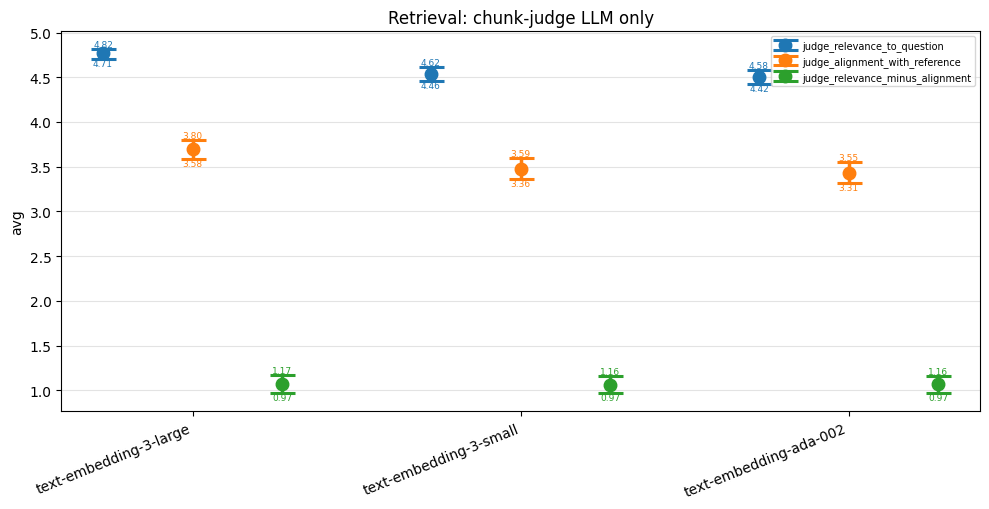
\includegraphics[width=\linewidth]{figures/retrieve-eval.png}
\caption{Визуализация метрик chunk-judge по трём моделям вложений (те же данные, что в табл.~\ref{tab:rag-chunk}).}
\label{fig:rag-retrieve-eval}
\end{figure}

Результаты (табл.~\ref{tab:rag-chunk} и рис.~\ref{fig:rag-retrieve-eval}) показывают, что модель \texttt{text-embedding-3-large} демонстрирует наилучшие показатели по всем ключевым метрикам. При этом наблюдается устойчивый разрыв между релевантностью и согласованностью, что указывает на склонность retrieval возвращать потенциально релевантные, но не всегда строго подтверждённые эталоном фрагменты.

\paragraph{Этап генерации}

На этапе генерации оценивались:
\begin{itemize}
\item соблюдение инструкции;
\item опора на переданные чанки;
\item корректность относительно контекста;
\item соответствие эталонному ответу.
\end{itemize}

\begin{table}[ht]
\centering
\caption{Answer-judge (генерация): среднее и 95\,\% ДИ бутстрапа, судья \texttt{gpt-4o}, фиксированный dense-retrieval (\texttt{text-embedding-3-large}, top-5; BM25 отключён). Источник: \texttt{evaluation\_bootstrap.ipynb}.}
\label{tab:rag-gen}
\small
\setlength{\tabcolsep}{2.5pt}
\begin{tabular}{|l|c|p{2.05cm}|p{2.05cm}|p{2.05cm}|p{2.05cm}|}
\hline
Генеративная модель & $n$ & Соблюдение инструкции & Верность чанкам & Корректность по чанкам & Соответствие эталону \\
\hline
\texttt{gpt-4o-mini} & 346 & 3{,}864 [3{,}754; 3{,}971] & 3{,}558 [3{,}436; 3{,}676] & 3{,}558 [3{,}436; 3{,}679] & 3{,}020 [2{,}887; 3{,}150] \\
\hline
\texttt{gpt-5.4} & 346 & 4{,}272 [4{,}165; 4{,}373] & 3{,}971 [3{,}853; 4{,}090] & 3{,}974 [3{,}855; 4{,}092] & 3{,}303 [3{,}185; 3{,}419] \\
\hline
\end{tabular}
\end{table}

\begin{figure}[ht]
\centering
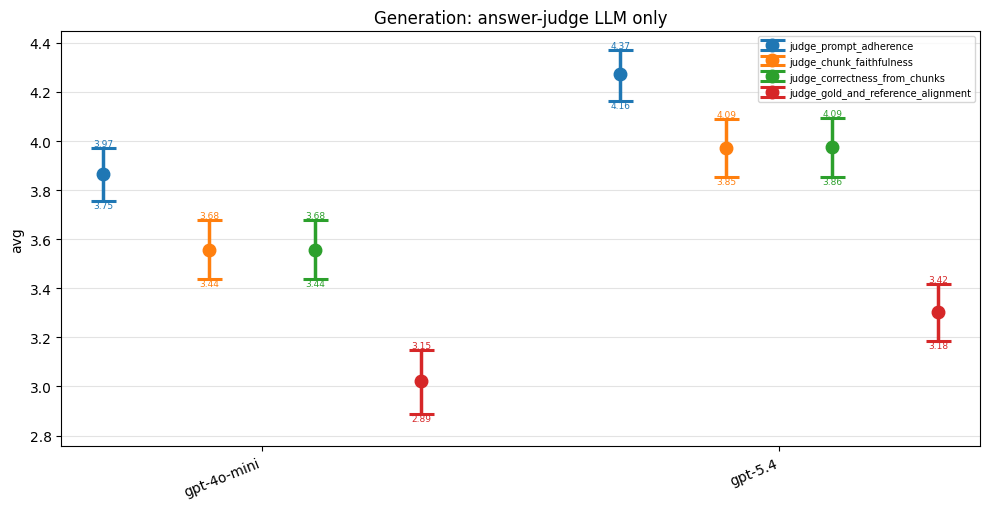
\includegraphics[width=\linewidth]{figures/gen-eval.png}
\caption{Визуализация метрик answer-judge для двух генеративных моделей (те же данные, что в табл.~\ref{tab:rag-gen}).}
\label{fig:rag-gen-eval}
\end{figure}

Сравнение моделей (табл.~\ref{tab:rag-gen} и рис.~\ref{fig:rag-gen-eval}) показывает, что модель \texttt{gpt-5.4} демонстрирует более высокие значения по всем метрикам, особенно по показателю соответствия эталону. Это подтверждает влияние качества генеративной модели при фиксированном retrieval.

\paragraph{Интерпретация результатов}

Полученные результаты позволяют сделать следующие выводы:
\begin{itemize}
\item качество retrieval является критическим фактором для итогового качества ответа;
\item улучшение генеративной модели повышает согласованность и точность;
\item существует компромисс между вычислительной стоимостью и качеством результата.
\end{itemize}

Полученные результаты согласуются с гипотезой о том, что опора генератора на извлекаемый по эмбеддингам контекст (dense-retrieval в Qdrant с последующей подстановкой чанков в промпт) повышает качество ответов по сравнению с изолированным использованием языковой модели без retrieval: это проявляется в более высоких значениях метрик, отражающих следование извлечённым фрагментам и согласованность с эталоном при фиксированной методике судейства (табл.~\ref{tab:rag-chunk}, \ref{tab:rag-gen}).

\subsubsection{Нагрузочное тестирование канала SignalR}

Для оценки устойчивости канала реального времени использован набор нагрузочных сценариев на базе клиента \texttt{@microsoft/signalr}. Тестирование выполнялось на изолированном стенде без записи в базу данных, что позволило измерить чистую пропускную способность транспортного уровня. Сводка численных результатов приведена в табл.~\ref{tab:loadtest-summary}; иллюстрации --- в рис.~\ref{fig:lt-flood}--\ref{fig:lt-hold}.

\paragraph{Сценарий \texttt{flood}}

Сценарий моделирует интенсивную нагрузку:
\[
100 \text{ клиентов} \times 20 \text{ сообщений/с} = 2000 \text{ сообщений/с}.
\]

В ходе теста зафиксировано:
\begin{itemize}
\item 59\,640 успешных сообщений;
\item средняя пропускная способность $\approx 1988$ сообщений/с;
\item $p_{50} \approx 6{,}07$ мс;
\item $p_{95} \approx 10{,}69$ мс;
\item $p_{99} \approx 15{,}71$ мс;
\item нарушений порядка доставки не обнаружено.
\end{itemize}

Полученные значения близки к теоретическому пределу, что указывает на отсутствие узких мест в обработке сообщений.

\paragraph{Сценарий \texttt{ping-series}}

Сценарий измеряет круговую задержку (RTT):
\begin{itemize}
\item 120 измерений;
\item медиана 3{,}90 мс;
\item $p_{95}$ 5{,}86 мс;
\item максимум 13{,}92 мс;
\item ошибок не зафиксировано.
\end{itemize}

Низкая вариативность задержек свидетельствует о стабильной работе канала.

\paragraph{Сценарий \texttt{hold}}

Сценарий проверяет устойчивость при длительном удержании соединений:
\begin{itemize}
\item 500 одновременных соединений;
\item длительность 600 с;
\item неожиданных разрывов: 0;
\item переподключений: 0.
\end{itemize}

Результаты подтверждают устойчивость системы при длительной нагрузке.

\begin{table}[ht]
\centering
\caption{Сводка нагрузочных сценариев SignalR (скриншоты консоли: \texttt{figures/loadtest-*.png}).}
\label{tab:loadtest-summary}
\small
\begin{tabular}{|l|p{4.2cm}|p{7.8cm}|}
\hline
Сценарий & Параметры запуска & Зафиксированные метрики \\
\hline
\texttt{flood} & 100 клиентов, 20 msg/s на клиента, 30~с, \texttt{parallel=20} & 59\,640 вызовов; пропускная способность $\approx 1988$~msg/s; $p_{50}{\approx}6{,}07$~мс, $p_{95}{\approx}10{,}69$~мс, $p_{99}{\approx}15{,}71$~мс; нарушений порядка~0 \\
\hline
\texttt{ping-series} & 120~с, интервал 1000~мс & 120 измерений RTT, сбоев~0; min 0{,}72~мс, $p_{50}$ 3{,}90~мс, $p_{95}$ 5{,}86~мс, max 13{,}92~мс \\
\hline
\texttt{hold} & 500 соединений, 600~с idle & Все 500 подключены; неожиданных разрывов~0; переподключений~0 \\
\hline
\end{tabular}
\end{table}

\begin{figure}[ht]
\centering
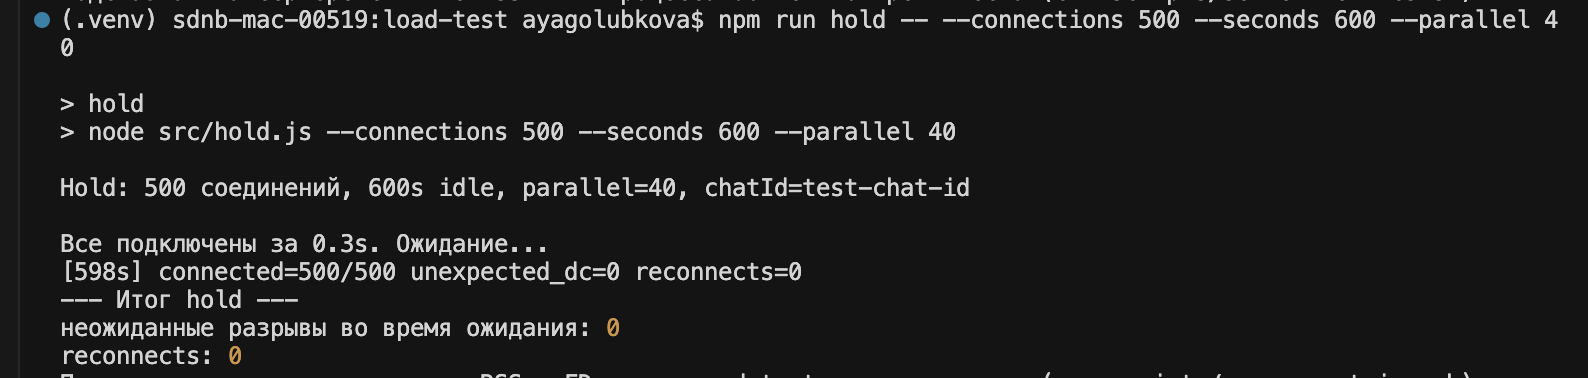
\includegraphics[width=\linewidth]{figures/loadtest-flood.png}
\caption{Консольный вывод сценария \texttt{flood}: пропускная способность и перцентили задержки.}
\label{fig:lt-flood}
\end{figure}

\begin{figure}[ht]
\centering
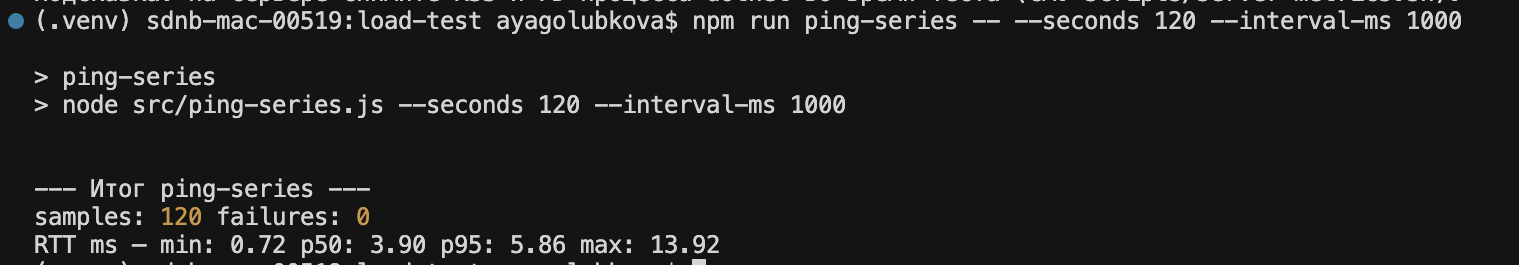
\includegraphics[width=\linewidth]{figures/loadtest-ping.png}
\caption{Консольный вывод сценария \texttt{ping-series}: статистика RTT.}
\label{fig:lt-ping}
\end{figure}

\begin{figure}[ht]
\centering
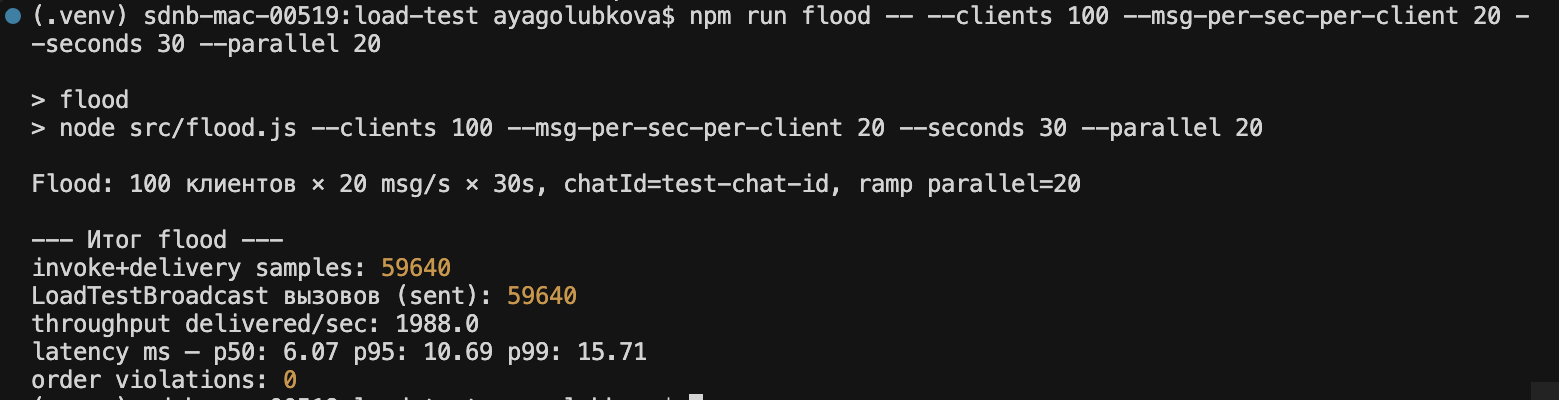
\includegraphics[width=\linewidth]{figures/loadtest-hold.png}
\caption{Консольный вывод сценария \texttt{hold}: удержание 500 соединений.}
\label{fig:lt-hold}
\end{figure}

\subsubsection{Выводы по результатам тестирования}

Проведённое тестирование показывает, что система:
\begin{itemize}
\item корректно реализует бизнес-логику и API;
\item демонстрирует устойчивую работу при интеграции компонентов;
\item обеспечивает приемлемое качество RAG-пайплайна;
\item в офлайн-оценке численные показатели согласуются с гипотезой о полезности dense-retrieval относительно генерации без извлечения контекста (при оговорённых ограничениях выборки и методики LLM-as-judge);
\item выдерживает высокую нагрузку в канале реального времени.
\end{itemize}

Таким образом, реализованная архитектура соответствует требованиям производительности, масштабируемости и надёжности.


% Список изученной литературы (все записи из bibl.bib)
\nocite{*}
\bibliographystyle{plainurl}
\bibliography{bibl}

\end{document}
